\chapter{7 TeV and 8 TeV Differential Cross Section Measurement: Systematic Uncertainties and Results}
\label{c:Differential_Cross_Section:systematics_and_results}

\section{Systematic uncertainties}
\label{s:systematic_uncertainties}
The systematic uncertainties in this analysis are evaluated by changing the inputs by the associated
uncertainties and measuring the change in the final result compared to the nominal measurement. The
uncertainty from a systematic source is then taken as the maximum value between the up or down systematic
variation. The total measurement error is obtained by adding the fitting, unfolding and systematic uncertainties in
quadrature.

In the case of experimental systematics, the uncertainty is calculated by changing the templates in the
fitting process and/or their normalisations, and using the nominal \MADGRAPH response matrix in the unfolding
process. In the case of theoretical systematics, the central fitting templates and normalisation are used,
while the response matrix information is changed according to the systematic being investigated.

The systematic uncertainties are summarised in Tables~\ref{tab:MET_systematics_7TeV_combined} to
\ref{tab:MT_systematics_8TeV_combined}.

\subsection{Experimental Uncertainties}
\label{ss:experimental_uncertainties}

Jet energy scale uncertainty is evaluated as a function of jet \pt and jet $\eta$ and a 10\% jet energy
resolution uncertainty is applied. The jet energy scale uncertainty becomes significant at higher values of
the primary variables, in particular of \met. This is because the jet energy corrections directly
affects the \met measurement by virtue of the jet energy corrections being propagated to the \met (see
Section~\ref{ss:met_corrections}). The \HT and \st variables are also affected, as the jet energy corrections
directly change the \pt of jets in the event.

Together with jet energy scale uncertainty, the \met energy uncertainties are the only systematics applied to
both simulation and data. These affect how the uncertainty on the energy of the lepton in the event affects
the \met. While the electron and muon energy uncertainties are not dominant sources of error in this analysis,
the tau energy has been calculated to be larger. Events with tau leptons can pass the signal selection (known
as fake events, i.e. non semi-leptonic \ttbar events which pass our signal selection) if they mimic the
signature of an electron+jets or muon+jets \ttbar event:

\begin{itemize}
 \item semi-leptonic tau, where $\tau \rightarrow e/\mu + \bar{\nu}_{e/\mu} + \nu_{\tau}$
 \item di-leptonic $e\tau$ \& $\mu\tau$, where $\tau \rightarrow q\bar{q}^{'} + \nu_\tau$
 \item di-leptonic $\tau\tau$, where $\tau \rightarrow q\bar{q}^{'} + \nu_\tau, \tau \rightarrow e/\mu
 + \bar{\nu}_{e/\mu}$
\end{itemize}

If, for example, the leptonically decaying \W boson from a semi-leptonic \ttbar decay decays to a tau lepton
and a tau neutrino, and the tau lepton then decays to another tau neutrino, an electron/muon and an
electron/muon neutrino via a virtual \W boson, such an event would fake our signal and pass the \ttbar signal
selection. Although the unfolding process removes fake events by subtracting the fake distribution obtained
from simulation, the shape of the fake distribution in the nominal measurement is also used to subtract from
the systematic measurements with the tau energy varied up and down. The comparison of shapes in the fake and
the signal distributions from \ttbar simulation are shown on the left in
Figure~\ref{fig:tau_shape_number_comparison}. It can be seen that relatively, the contribution from fakes
increases as \met increases. The effect of varying the electron and muon energies is not so pronounced because
there are not many electrons or muons in the fake collection (a dileptonic \ttbar event with $ee$, $e\mu$ or
$\mu\mu$ would have to be misreconstructed as a semi-leptonic event for this to happen). However, since
approximately 14\% of the reconstructed \ttbar events in simulation are fake events (13.5\% in electron
channel and 13.9\% in muon channel), as seen on the right in Figure~\ref{fig:tau_shape_number_comparison},
varying the tau energy has a more significant influence on the measurement.

\begin{figure}[hbtp]
    \centering
     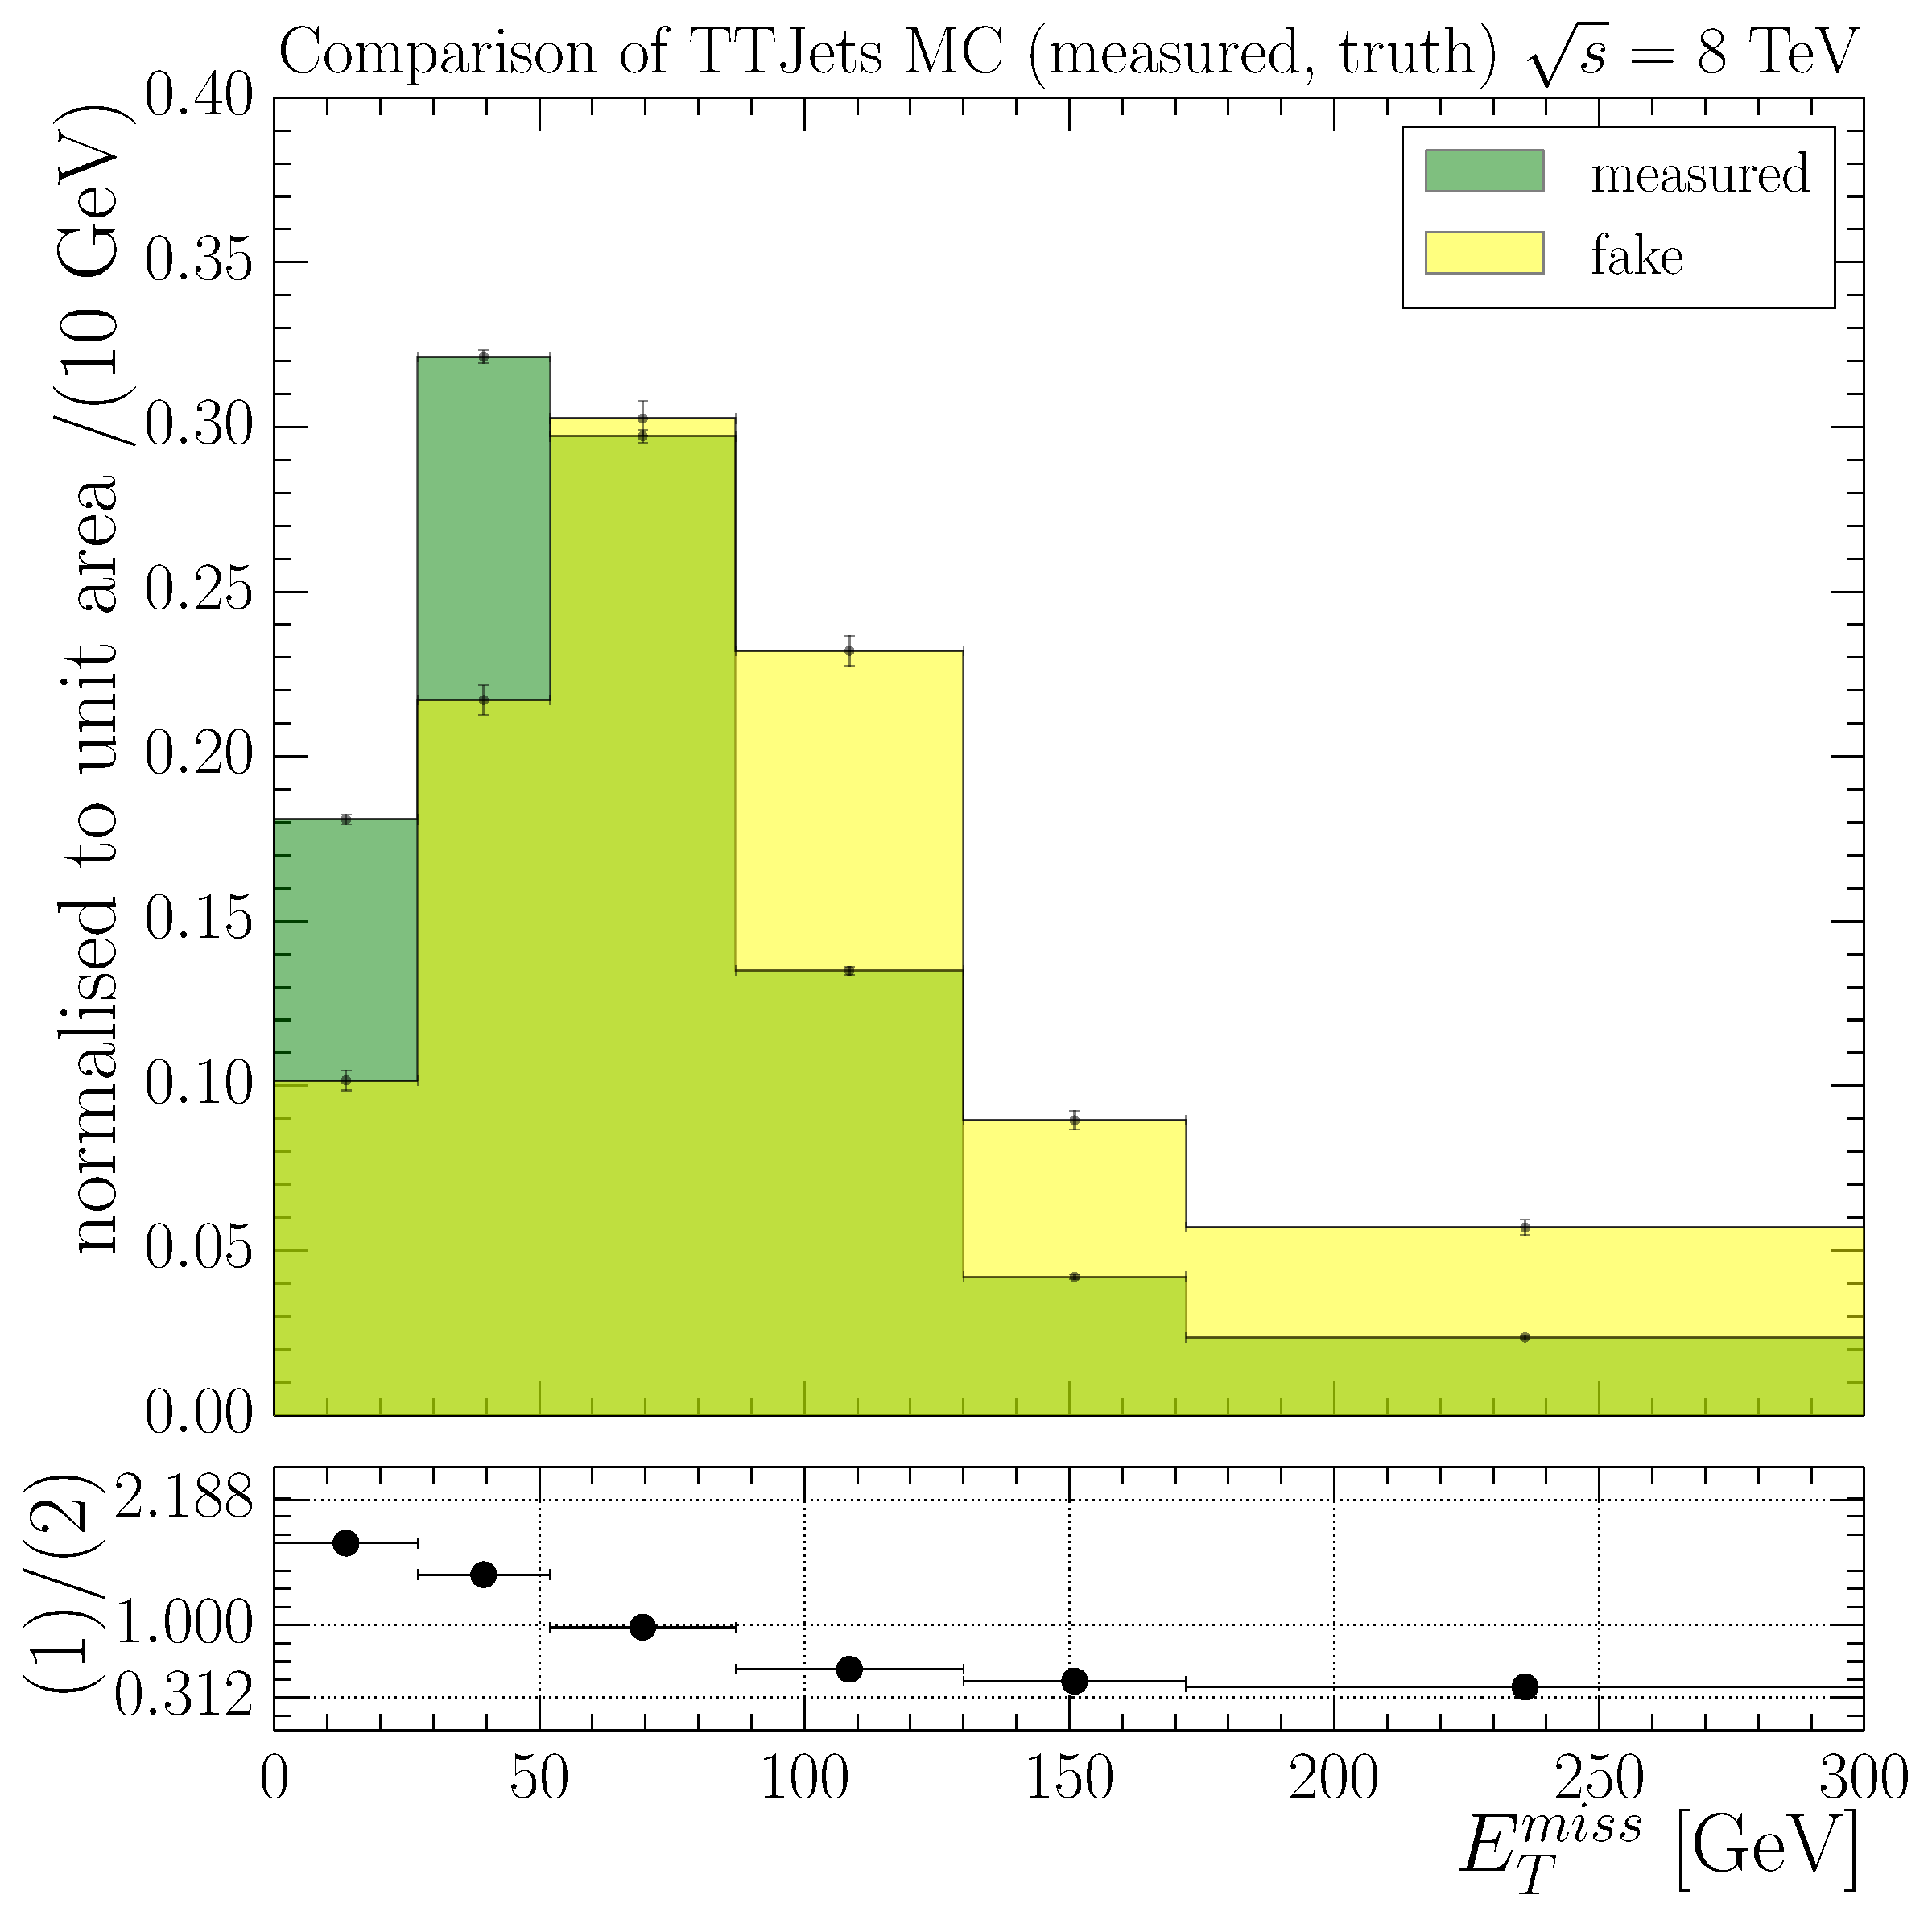
\includegraphics[width=0.48\textwidth]{Chapters/04_Analysis/04b_XSections/images/tau_cross_checks/comparison_measured_fakeTTJets_normalised_to_one.pdf}\hfill
     % \includegraphics[width=0.48\textwidth]{Chapters/04_Analysis/04b_XSections/images/tau_cross_checks/comparison_measured_fakeTTJets.pdf}
     
\includegraphics[width=0.48\textwidth]{Chapters/04_Analysis/04b_XSections/images/placeholder.png}
\caption{Comparison of the signal and fake distributions from semi-leptonic \ttbar events after
     selection in simulation in the electron+jets channel at $\roots=8\TeV$ normalised to one (left) and
     normalised to the numbers of events (right). TODO:MAKE SECOND PLOT} %TODO:MAKE SECOND PLOT
     \label{fig:tau_shape_number_comparison}
\end{figure}

The difference between the tau energy down ($-1\sigma$) variation and the nominal measurements in the \met
variable before fitting and unfolding is shown in Figure~\ref{fig:tau_down_comparison}. In the highest \met
bin, the difference is approximately 6\%, and this value remains approximately constant after fitting and
unfolding, as shown in Table~\ref{tab:tau_up_down_final_bin_comparison}. It can be seen therefore that the
significant affect of varying the tau energy is not an artifact of the fitting and/or unfolding procedure, but
a real difference in the number of events.

\begin{figure}[hbtp]
    \centering
     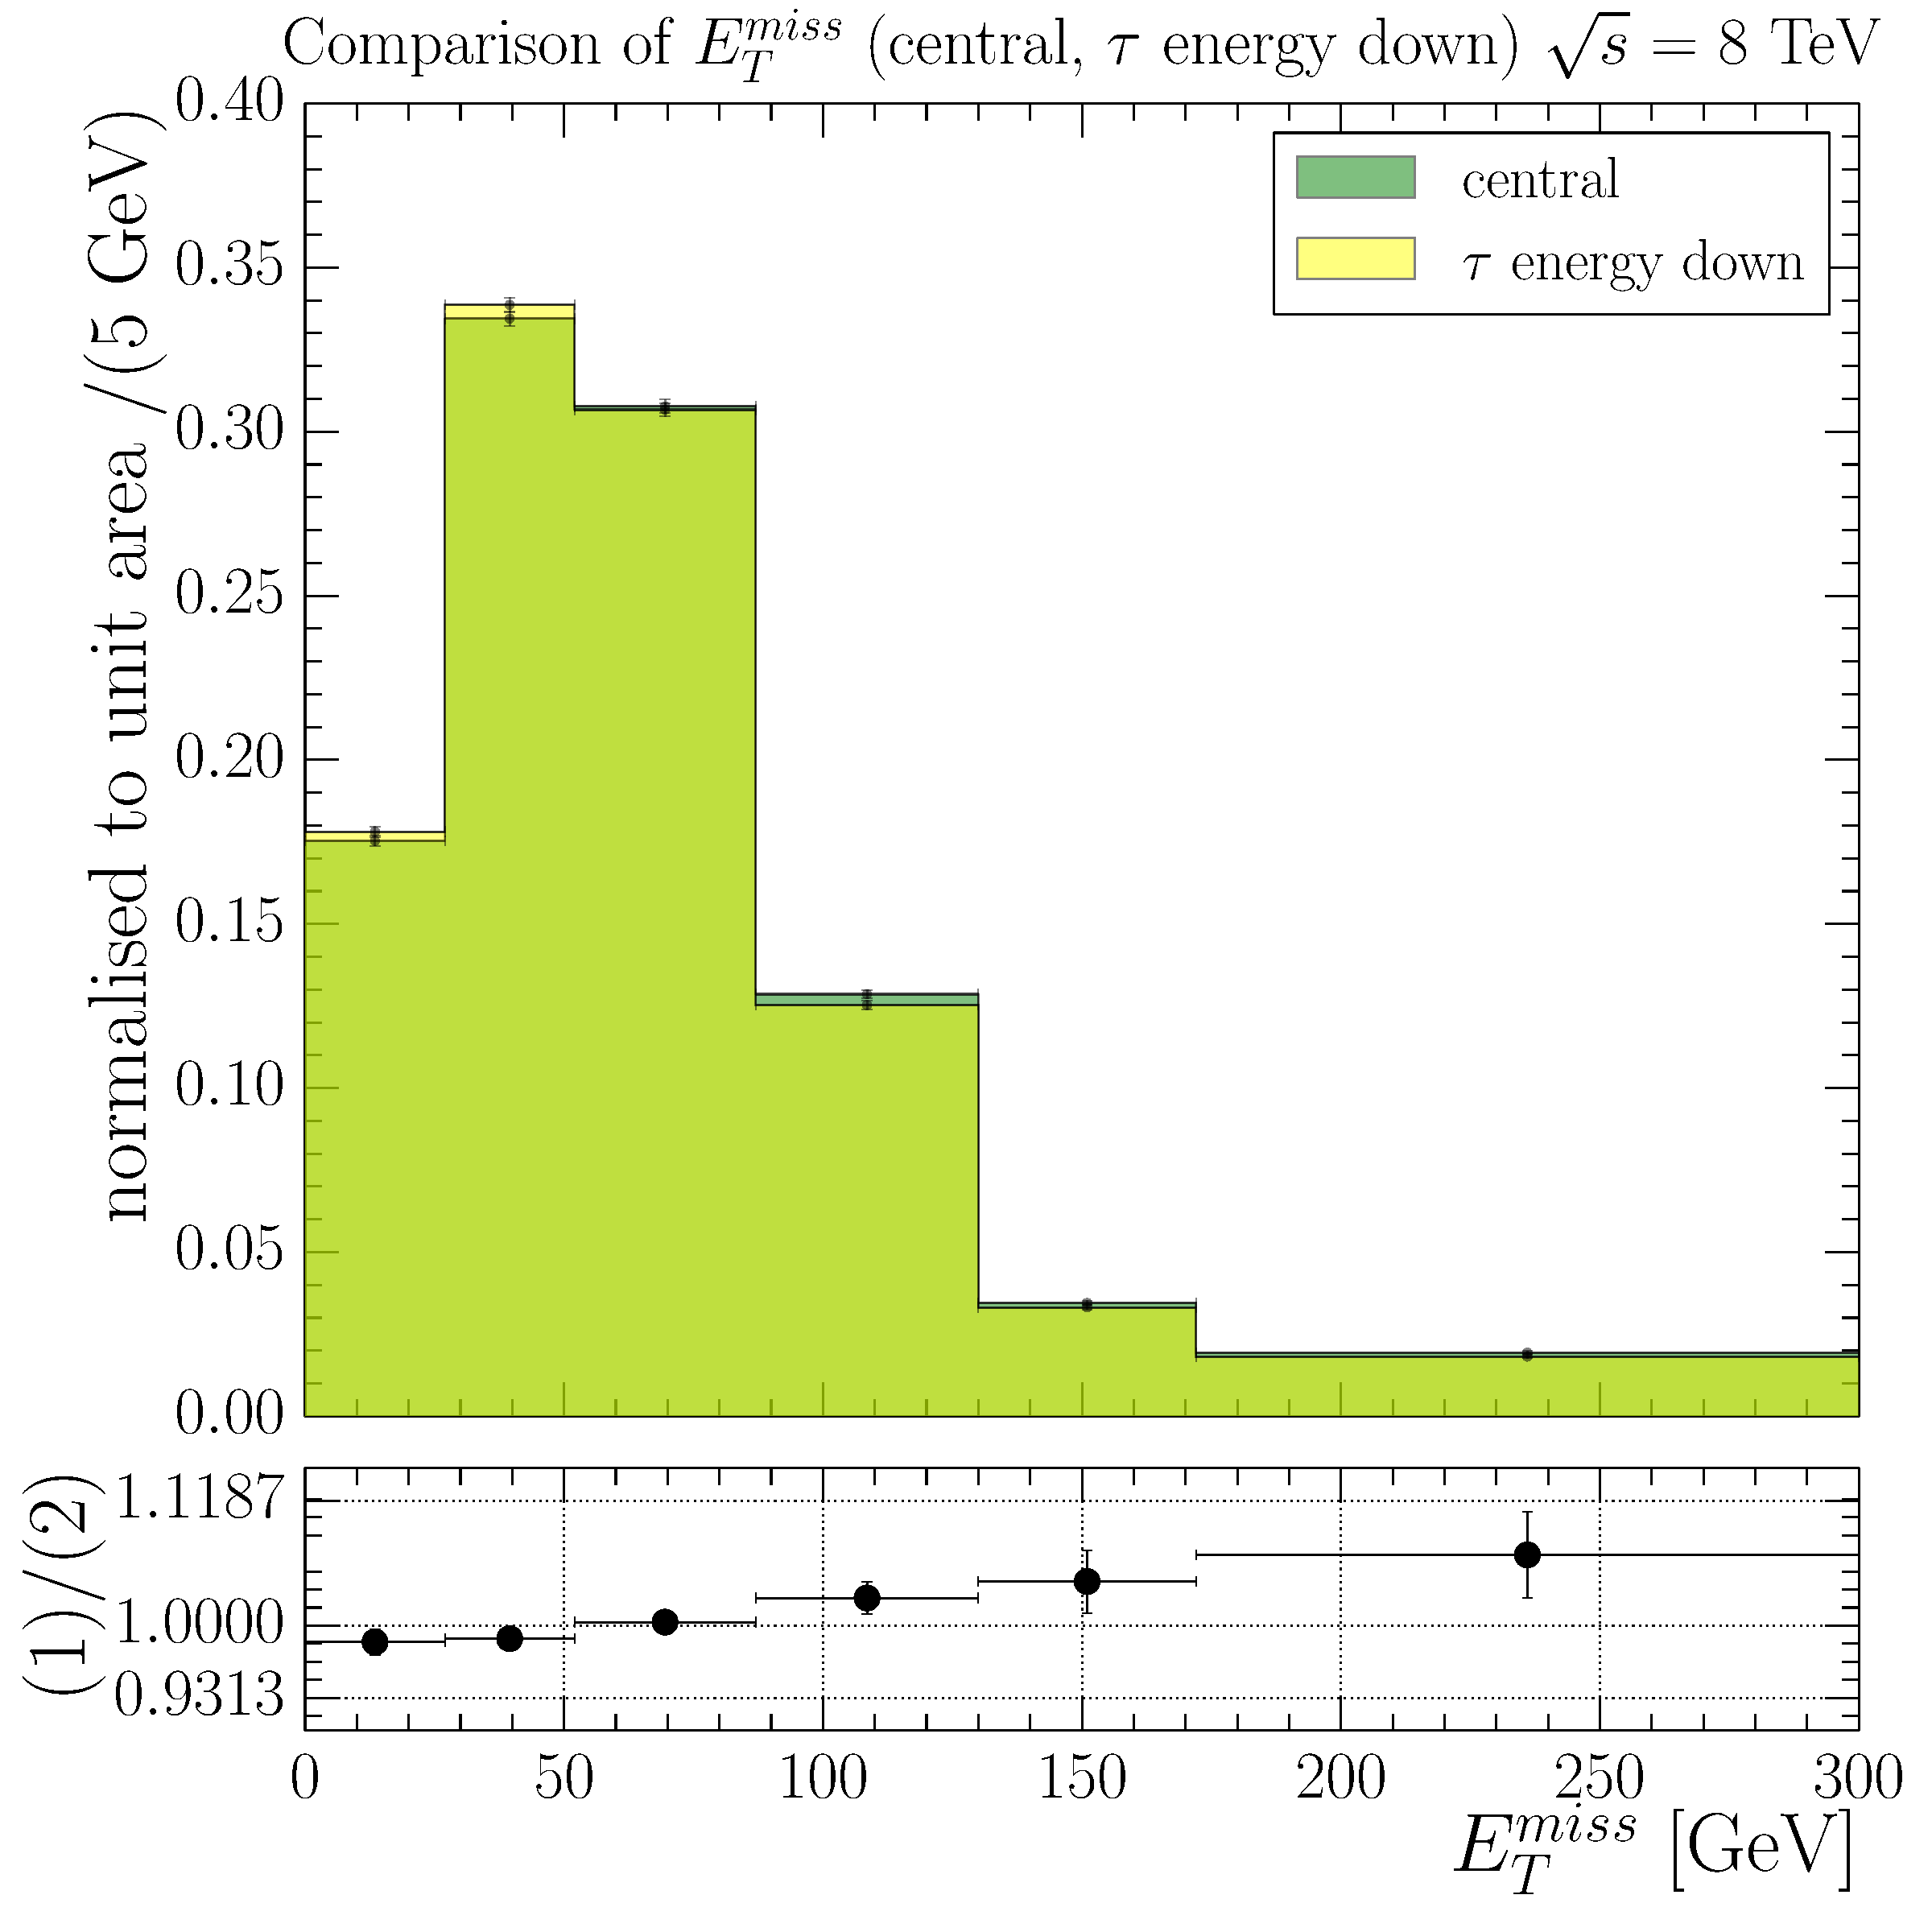
\includegraphics[width=0.48\textwidth]{Chapters/04_Analysis/04b_XSections/images/tau_cross_checks/compare_central_MET_to_tau_energy_down_asym_bins_electron_channel_data.pdf}\hfill
     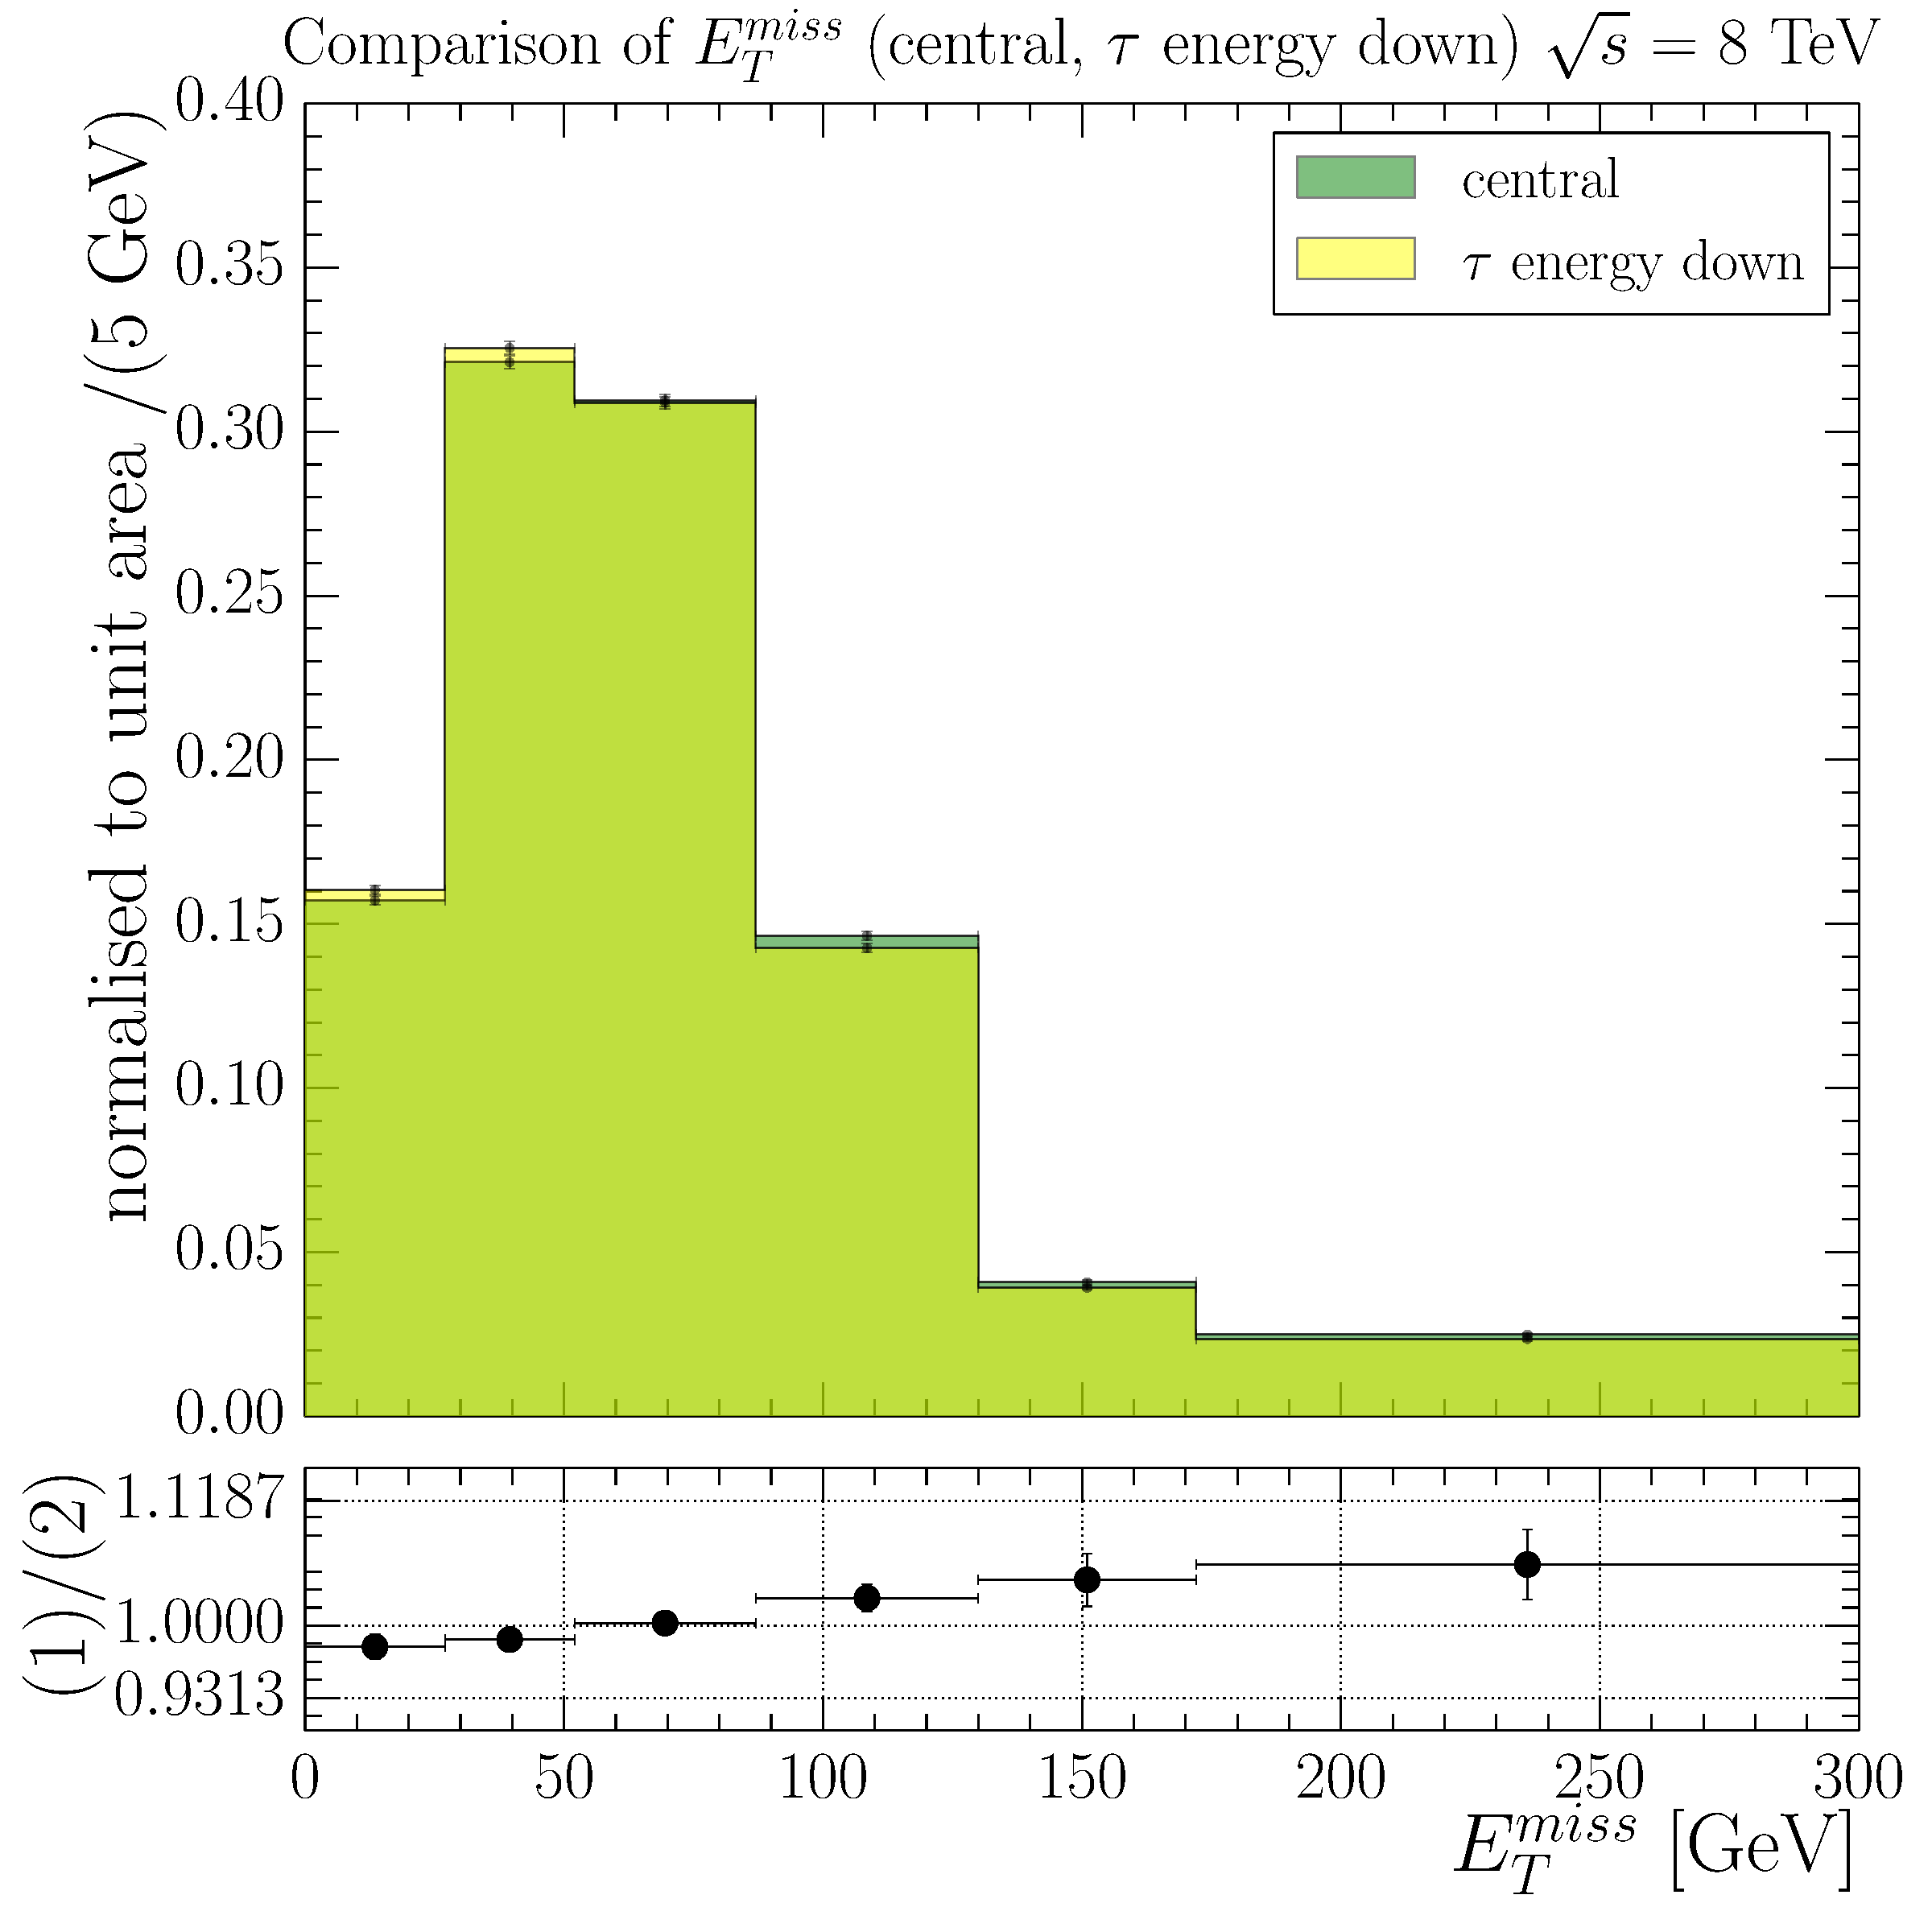
\includegraphics[width=0.48\textwidth]{Chapters/04_Analysis/04b_XSections/images/tau_cross_checks/compare_central_MET_to_tau_energy_down_asym_bins_electron_channel_TTJet.pdf}
     \caption{Comparison of the \met distributions in the nominal measurement and in the tau energy down
     variation before fitting and unfolding in data (left) and in \ttbar simulation (right) at
     $\roots=8\TeV$}
     \label{fig:tau_down_comparison}
\end{figure}
 
%% ============================================================
% Difference between central and tau energy up and down systematic value in highest \met bin
%% ============================================================
\begin{table}[htbp]
\centering
\caption{Difference between central and tau energy up and down systematic value in highest \met bin at a
centre-of-mass energy of 8 TeV in the electron channel TODO: FILL TABLE} %TODO: FILL TABLE
\label{tab:tau_up_down_final_bin_comparison}
\resizebox{\columnwidth}{!} {
\begin{tabular}{lrr}
\hline
Stage & $\tau$ energy up & $\tau$ energy down \\
\hline
Before Fitting \& Unfolding(\%) & & \\
After Fitting, before Unfolding(\%) & & \\
After Fitting \& Unfolding(\%) & & \\
\hline
\end{tabular}
}
\end{table}


Other small sources of experimental uncertainty include the non-clustered energy uncertainty (which refers to
the fluctuations in deposits in the electromagnetic calorimeter that are not included in jet clusters), the
matching threshold and factorisation and normalisation scale uncertainties in \WpJets and \ZpJets events,
pileup uncertainty, the QCD template shape uncertainty, and the efficiency of electron, muon and \btagging in
the selection process.

The tau energy systematic becomes more significant in the region of higher primary variable values. This stems
from \ttbar events with tau leptons. Taus could pass the signal selection in two ways. Events in which one \W
boson decays to a muon or an electron and the associated neutrino, and the other \W boson decays to a $\tau$
lepton which then decays hadronically; and also semi-leptonic events in which the lepton is a tau, which then
decays to a tau neutrino, and electron or a muon and the associated neutrino. This 

Rate changing systematics such as the uncertainty on the luminosity and the uncertainty on the theoretical
cross-sections of the signal and background processes have a negligible effect on the final result, since they
influence only the template normalisations that are input to the fitting process.

\subsection{Theoretical Uncertainties}
\label{ss:theoretical_uncertainties}

The factorisation and normalisation scale ($Q^{2}$ up/down) uncertainty is evaluated using simulation samples
produced with the scale varied by factors of 2 (up) and 0.5 (down). This has been evaluated to be one of the
dominating uncertainties in this analysis. The uncertainty in the matching theshold (matching up/down) for
\ttbar events is evaluated in the same way.

The uncertainty due to hadronisation modelling is evaluated by comparing a simulated sample
generated using the \POWHEG generator and \PYTHIA to model the hadron showering (\POWHEG+\PYTHIA) to a sample
generator using the same \POWHEG generator and \HERWIG to model the hadron showering (\POWHEG+\HERWIG). The
difference between the \PYTHIA and \HERWIG samples is scaled to the nominal measurement and taken as the
hadronisation uncertainty. All variables, and in particular those sensitive to hadronic aspects of an event
such as \HT and \st, are significantly affected by this systematic, with a larger uncertainty at lower
values of the primary variables. %\a MADGRAPH+HERWIG sample was not available.

The proton PDF uncertainties are evaluated similarly, with 44 distinct weights from the CTEQ 6.6 PDF sets used
to reweight events in the simulated samples and repeat the analysis.
Top quark mass uncertainty is evaluated using \ttbar samples produced with two different top quark masses of
169.5\GeV and 173.5\GeV, and scaling the the error obtained using these samples to the top mass uncertainty of
$\pm1.0\GeV$.

There is a known problem with event generators mismodelling the top quark \pt distribution; the distribution
of the transverse momentum of top quarks in data was found to be softer than that in simulation
\cite{Chatrchyan:2012saa}. The effect of this correction on the nominal measurement was evaluated to be
negligible for low values of the primary variables, increasing to 3-7\% at higher values. The \MADGRAPH
simulation after applying the \tquark \pt correction is also included in the results plots
(Figures~\ref{fig:result_MET_7TeV_combined} to \ref{fig:result_WPT_8TeV_combined}).

The most significant shape changing uncertainties typically arise from the factorisation scale variations in
the \ttbar process and the hadronisation.

\subsection{Systematic Uncertainty Tables}
\label{ss:systematic_uncertainty_tables}

%% ============================================================
% Systematics table for MET variable, combined channel, k-value None, met type patType1CorrectedPFMet, 2orMoreBtags b-tag region
%% ============================================================
\begin{table}[htbp]
\centering
\caption{Systematic uncertainties for the normalised \ttbar cross section measurement with respect to \MET variable
at a centre-of-mass energy of 7 TeV (combination of electron and muon channels).}
\label{tab:MET_systematics_7TeV_combined}
\resizebox{\columnwidth}{!} {
\begin{tabular}{lrrrrrr}
\hline
Uncertainty source & 0--27~\GeV& 27--52~\GeV& 52--87~\GeV& 87--130~\GeV& 130--172~\GeV& $\geq 172$~\GeV \\
\hline
b-tagging efficiency $-1\sigma$ (\%) & -0.08 & -0.04 & 0.02 & 0.09 & 0.14 & 0.18 \\ 
b-tagging efficiency $+1\sigma$ (\%) & -0.03 & -0.02 & 0.01 & 0.04 & 0.07 & 0.09 \\ 
Electron efficiency $-1\sigma$ (\%) & -0.11 & -0.04 & 0.04 & 0.10 & 0.14 & 0.17 \\ 
Electron efficiency $+1\sigma$ (\%) & -0.25 & -0.10 & 0.09 & 0.24 & 0.37 & 0.49 \\ 
Jet energy resolution $-1\sigma$ (\%) & -0.10 & -0.03 & 0.04 & 0.08 & 0.10 & 0.11 \\ 
Jet energy resolution $+1\sigma$ (\%) & -0.38 & -0.15 & 0.14 & 0.36 & 0.50 & 0.60 \\ 
Jet energy scale $-1\sigma$ (\%) & 0.00 & -0.01 & -0.01 & 0.03 & 0.05 & 0.04 \\ 
Jet energy scale $+1\sigma$ (\%) & 0.00 & 0.00 & 0.00 & -0.01 & -0.03 & -0.06 \\ 
Muon efficiency $-1\sigma$ (\%) & -0.00 & -0.00 & 0.00 & 0.00 & 0.00 & 0.01 \\ 
Muon efficiency $+1\sigma$ (\%) & 0.00 & 0.00 & -0.00 & -0.00 & -0.00 & -0.01 \\ 
PDF uncertainty $-1\sigma$ (\%) & 1.50 & 0.72 & 0.65 & 0.97 & 0.78 & 2.02 \\ 
PDF uncertainty $+1\sigma$ (\%) & 1.50 & 0.72 & 0.65 & 0.97 & 0.78 & 2.02 \\ 
Pile-up $-1\sigma$ (\%) & -0.24 & -0.07 & 0.11 & 0.19 & 0.21 & 0.21 \\ 
Pile-up $+1\sigma$ (\%) & -0.16 & -0.07 & 0.05 & 0.16 & 0.26 & 0.33 \\ 
QCD shape uncertainty (\%) & 0.04 & 0.02 & -0.01 & -0.05 & -0.10 & -0.14 \\ 
Single top cross section $+1\sigma$ (\%) & 0.00 & 0.00 & -0.00 & -0.00 & -0.00 & -0.00 \\ 
Single top cross section $-1\sigma$ (\%) & -0.00 & -0.00 & 0.00 & 0.00 & 0.00 & 0.00 \\ 
$t\bar{t}$ cross section $+1\sigma$ (\%) & -0.00 & -0.00 & 0.00 & 0.00 & 0.00 & 0.00 \\ 
$t\bar{t}$ cross section $-1\sigma$ (\%) & -0.00 & -0.00 & 0.00 & 0.00 & 0.00 & 0.00 \\ 
$t\bar{t}$ (top mass down) (\%) & 0.05 & -0.05 & 0.03 & -0.09 & 0.34 & -0.05 \\ 
$t\bar{t}$ (top mass up) (\%) & -0.12 & 0.08 & 0.36 & -0.65 & -0.85 & -0.05 \\ 
$t\bar{t}$ (matching down) (\%) & -0.08 & 0.18 & 0.02 & -0.70 & -0.15 & 2.54 \\ 
$t\bar{t}$ (matching up) (\%) & -0.11 & -0.10 & 0.39 & -0.03 & -0.93 & -1.59 \\ 
$t\bar{t}$ ($Q^{2}$ down) (\%) & -0.08 & 0.12 & 0.25 & -0.54 & -0.41 & -1.18 \\ 
$t\bar{t}$ ($Q^{2}$ up) (\%) & -0.66 & 0.03 & 0.47 & -0.33 & 0.09 & 0.47 \\ 
V+jets (matching down) (\%) & -0.45 & -0.21 & 0.15 & 0.49 & 0.77 & 0.98 \\ 
V+jets (matching up) (\%) & -0.47 & -0.20 & 0.17 & 0.47 & 0.66 & 0.79 \\ 
V+jets ($Q^{2}$ down) (\%) & -0.65 & -0.30 & 0.22 & 0.70 & 1.07 & 1.35 \\ 
V+jets ($Q^{2}$ up) (\%) & -0.56 & -0.26 & 0.19 & 0.61 & 0.93 & 1.16 \\ 
Hadronisation uncertainty (\%) & 1.11 & 1.29 & 0.14 & 2.87 & 6.27 & 7.37 \\ 
Luminosity $+1\sigma$ (\%) & -0.00 & -0.00 & 0.00 & 0.00 & 0.00 & 0.00 \\ 
Luminosity $-1\sigma$ (\%) & 0.00 & 0.00 & -0.00 & -0.00 & -0.00 & -0.00 \\ 
Electron energy $-1\sigma$ (\%) & -0.21 & -0.10 & 0.06 & 0.24 & 0.39 & 0.51 \\ 
Electron energy $+1\sigma$ (\%) & -0.34 & -0.13 & 0.13 & 0.31 & 0.42 & 0.49 \\ 
Muon energy $-1\sigma$ (\%) & 0.01 & 0.00 & -0.01 & -0.01 & -0.01 & -0.01 \\ 
Muon energy $+1\sigma$ (\%) & -0.00 & 0.00 & 0.00 & -0.00 & -0.01 & -0.02 \\ 
Tau energy $-1\sigma$ (\%) & 1.04 & 0.56 & -0.28 & -1.25 & -2.20 & -2.96 \\ 
Tau energy $+1\sigma$ (\%) & -1.41 & -0.76 & 0.36 & 1.72 & 3.03 & 4.06 \\ 
Unclustered energy $-1\sigma$ (\%) & 0.01 & 0.09 & 0.06 & -0.16 & -0.46 & -0.73 \\ 
Unclustered energy $+1\sigma$ (\%) & -0.36 & -0.19 & 0.09 & 0.44 & 0.80 & 1.07 \\ 
$p_\mathrm{T}(t,\bar{t})$ reweighting (\%) & 0.94 & 1.42 & 1.44 & 2.00 & 6.66 & 14.90 \\ 
\hline 
Total (\%) & 3.42  & 2.63  & 2.29  & 4.73  & 10.33  & 17.91 \\ 
\hline 
\end{tabular}
}
\end{table}

\begin{landscape}
%% ============================================================
% Systematics table for HT variable, combined channel, k-value None, met type patType1CorrectedPFMet, 2orMoreBtags b-tag region
%% ============================================================
\begin{table}[htbp]
\centering
\caption{Systematic uncertainties for the normalised \ttbar cross section measurement with respect to \HT variable
at a centre-of-mass energy of 7 TeV (combination of electron and muon channels).}
\label{tab:HT_systematics_7TeV_combined}
\resizebox{\columnwidth}{!} {
\begin{tabular}{lrrrrrrrrrrrrrr}
\hline
Uncertainty source & 120--185~\GeV& 185--215~\GeV& 215--247~\GeV& 247--283~\GeV& 283--323~\GeV& 323--365~\GeV& 365--409~\GeV& 409--458~\GeV& 458--512~\GeV& 512--570~\GeV& 570--629~\GeV& 629--691~\GeV& 691--769~\GeV& $\geq 769$~\GeV \\
\hline
b-tagging efficiency $-1\sigma$ (\%) & -0.08 & -0.08 & -0.09 & -0.09 & -0.03 & 0.06 & 0.15 & 0.24 & 0.31 & 0.38 & 0.42 & 0.45 & 0.47 & 0.48 \\ 
b-tagging efficiency $+1\sigma$ (\%) & 0.08 & 0.09 & 0.09 & 0.08 & 0.02 & -0.06 & -0.16 & -0.24 & -0.31 & -0.36 & -0.40 & -0.42 & -0.43 & -0.44 \\ 
Electron efficiency $-1\sigma$ (\%) & 1.17 & 1.12 & 0.99 & 0.64 & -0.11 & -1.02 & -1.86 & -2.52 & -2.99 & -3.31 & -3.51 & -3.62 & -3.69 & -3.73 \\ 
Electron efficiency $+1\sigma$ (\%) & 0.88 & 0.87 & 0.81 & 0.59 & 0.01 & -0.79 & -1.56 & -2.13 & -2.53 & -2.76 & -2.87 & -2.91 & -2.92 & -2.93 \\ 
Jet energy resolution $-1\sigma$ (\%) & -0.68 & -0.53 & -0.23 & 0.15 & 0.46 & 0.65 & 0.70 & 0.63 & 0.48 & 0.30 & 0.12 & -0.04 & -0.19 & -0.28 \\ 
Jet energy resolution $+1\sigma$ (\%) & 0.04 & 0.00 & -0.05 & -0.07 & -0.08 & -0.07 & -0.07 & -0.07 & -0.01 & 0.15 & 0.46 & 0.89 & 1.35 & 1.65 \\ 
Jet energy scale $-1\sigma$ (\%) & 2.91 & 2.54 & 1.80 & 0.65 & -0.80 & -2.26 & -3.64 & -4.77 & -5.55 & -6.03 & -6.23 & -6.19 & -6.07 & -5.91 \\ 
Jet energy scale $+1\sigma$ (\%) & 0.97 & 0.60 & 0.05 & -0.54 & -1.02 & -1.22 & -1.10 & -0.69 & 0.10 & 1.23 & 2.57 & 3.86 & 4.96 & 5.80 \\ 
Muon efficiency $-1\sigma$ (\%) & 0.01 & 0.01 & 0.01 & -0.00 & -0.01 & -0.02 & -0.02 & -0.02 & -0.01 & 0.01 & 0.02 & 0.04 & 0.05 & 0.07 \\ 
Muon efficiency $+1\sigma$ (\%) & -0.00 & -0.00 & -0.00 & 0.00 & 0.00 & 0.01 & 0.01 & 0.00 & -0.00 & -0.01 & -0.02 & -0.02 & -0.03 & -0.04 \\ 
PDF uncertainty $-1\sigma$ (\%) & 0.78 & 0.35 & 0.38 & 0.50 & 0.48 & 0.86 & 0.73 & 0.77 & 0.92 & 1.11 & 1.35 & 1.52 & 1.68 & 1.28 \\ 
PDF uncertainty $+1\sigma$ (\%) & 0.78 & 0.35 & 0.38 & 0.50 & 0.48 & 0.86 & 0.73 & 0.77 & 0.92 & 1.11 & 1.35 & 1.52 & 1.68 & 1.28 \\ 
Pile-up $-1\sigma$ (\%) & -0.09 & -0.03 & 0.06 & 0.12 & 0.09 & 0.01 & -0.07 & -0.12 & -0.14 & -0.15 & -0.14 & -0.12 & -0.13 & -0.14 \\ 
Pile-up $+1\sigma$ (\%) & 0.03 & 0.03 & 0.04 & 0.05 & 0.05 & 0.01 & -0.06 & -0.16 & -0.22 & -0.27 & -0.26 & -0.20 & -0.13 & -0.06 \\ 
QCD shape uncertainty (\%) & 0.11 & 0.10 & 0.07 & 0.03 & -0.02 & -0.08 & -0.15 & -0.18 & -0.21 & -0.25 & -0.29 & -0.34 & -0.41 & -0.47 \\ 
Single top cross section $+1\sigma$ (\%) & 0.13 & 0.13 & 0.11 & 0.08 & -0.01 & -0.12 & -0.22 & -0.29 & -0.34 & -0.37 & -0.39 & -0.39 & -0.39 & -0.39 \\ 
Single top cross section $-1\sigma$ (\%) & 0.10 & 0.10 & 0.08 & 0.05 & -0.01 & -0.10 & -0.17 & -0.22 & -0.25 & -0.26 & -0.26 & -0.26 & -0.25 & -0.25 \\ 
$t\bar{t}$ cross section $+1\sigma$ (\%) & 0.05 & 0.05 & 0.04 & 0.03 & -0.01 & -0.05 & -0.09 & -0.11 & -0.13 & -0.13 & -0.13 & -0.13 & -0.13 & -0.13 \\ 
$t\bar{t}$ cross section $-1\sigma$ (\%) & -0.06 & -0.06 & -0.06 & -0.04 & 0.00 & 0.06 & 0.11 & 0.14 & 0.17 & 0.19 & 0.20 & 0.20 & 0.21 & 0.21 \\ 
$t\bar{t}$ (top mass down) (\%) & 0.01 & 0.04 & -0.06 & 0.10 & -0.14 & 0.19 & -0.04 & -0.10 & 0.07 & -0.19 & -0.53 & 0.05 & 0.28 & 0.13 \\ 
$t\bar{t}$ (top mass up) (\%) & -0.47 & 0.30 & -0.31 & 0.56 & 0.03 & 0.13 & 0.10 & -0.30 & -0.54 & -0.13 & 0.12 & 0.84 & 0.49 & -0.12 \\ 
$t\bar{t}$ (matching down) (\%) & -1.30 & -0.27 & -0.53 & 0.55 & 0.49 & 0.71 & 0.50 & 1.90 & 0.63 & 0.35 & 0.74 & 0.77 & -0.97 & -2.91 \\ 
$t\bar{t}$ (matching up) (\%) & -1.26 & -0.38 & 0.02 & 0.86 & 0.13 & 0.21 & 0.19 & 0.92 & 0.15 & 0.00 & -0.34 & 0.12 & 1.55 & 4.26 \\ 
$t\bar{t}$ ($Q^{2}$ down) (\%) & -7.75 & -4.31 & -0.96 & 2.05 & 3.36 & 4.97 & 5.30 & 5.07 & 4.71 & 4.66 & 3.00 & 2.75 & 3.06 & 2.63 \\ 
$t\bar{t}$ ($Q^{2}$ up) (\%) & 5.18 & 2.51 & 0.06 & -0.92 & -2.83 & -2.92 & -3.40 & -2.58 & -2.17 & -2.19 & -2.10 & -2.25 & 0.74 & -0.11 \\ 
V+jets (matching down) (\%) & -1.14 & -1.01 & -0.74 & -0.29 & 0.30 & 0.94 & 1.50 & 1.94 & 2.21 & 2.37 & 2.45 & 2.45 & 2.43 & 2.40 \\ 
V+jets (matching up) (\%) & -0.50 & -0.39 & -0.16 & 0.14 & 0.37 & 0.50 & 0.52 & 0.46 & 0.31 & 0.11 & -0.09 & -0.27 & -0.44 & -0.56 \\ 
V+jets ($Q^{2}$ down) (\%) & -1.13 & -0.97 & -0.65 & -0.20 & 0.29 & 0.80 & 1.29 & 1.73 & 2.08 & 2.34 & 2.51 & 2.59 & 2.60 & 2.58 \\ 
V+jets ($Q^{2}$ up) (\%) & -0.59 & -0.49 & -0.27 & 0.00 & 0.25 & 0.47 & 0.67 & 0.82 & 0.88 & 0.83 & 0.70 & 0.56 & 0.43 & 0.34 \\ 
Hadronisation uncertainty (\%) & 36.00 & 13.05 & 3.07 & 10.70 & 12.57 & 13.68 & 12.30 & 10.71 & 9.24 & 10.27 & 7.61 & 6.30 & 5.55 & 1.61 \\ 
Luminosity $+1\sigma$ (\%) & 0.04 & 0.04 & 0.03 & 0.02 & 0.00 & -0.03 & -0.05 & -0.08 & -0.11 & -0.13 & -0.15 & -0.16 & -0.17 & -0.18 \\ 
Luminosity $-1\sigma$ (\%) & -0.05 & -0.05 & -0.05 & -0.03 & 0.00 & 0.04 & 0.08 & 0.11 & 0.14 & 0.16 & 0.18 & 0.19 & 0.20 & 0.20 \\ 
$p_\mathrm{T}(t,\bar{t})$ reweighting (\%) & 1.67 & 0.61 & 0.23 & 0.86 & 1.05 & 0.83 & 0.38 & 0.21 & 0.66 & 0.91 & 1.00 & 0.69 & 0.05 & 4.78 \\ 
\hline 
Total (\%) & 37.19  & 14.40  & 4.78  & 11.32  & 13.33  & 15.08  & 14.36  & 13.62  & 12.73  & 13.87  & 11.88  & 11.30  & 11.36  & 11.80 \\ 
\hline 
\end{tabular}
}
\end{table}

\end{landscape}
\begin{landscape}
%% ============================================================
% Systematics table for ST variable, combined channel, k-value None, met type patType1CorrectedPFMet, 2orMoreBtags b-tag region
%% ============================================================
\begin{table}[htbp]
\centering
\caption{Systematic uncertainties for the normalised \ttbar cross section measurement with respect to \ST variable
at a centre-of-mass energy of 7 TeV (combination of electron and muon channels).}
\label{tab:ST_systematics_7TeV_combined}
\resizebox{\columnwidth}{!} {
\begin{tabular}{lrrrrrrrrrrrrr}
\hline
Uncertainty source & 146--277~\GeV& 277--319~\GeV& 319--361~\GeV& 361--408~\GeV& 408--459~\GeV& 459--514~\GeV& 514--573~\GeV& 573--637~\GeV& 637--705~\GeV& 705--774~\GeV& 774--854~\GeV& 854--940~\GeV& $\geq 940$~\GeV \\
\hline
b-tagging efficiency $-1\sigma$ (\%) & 0.05 & 0.05 & 0.04 & 0.02 & -0.03 & -0.09 & -0.17 & -0.21 & -0.20 & -0.12 & 0.06 & 0.27 & 0.46 \\ 
b-tagging efficiency $+1\sigma$ (\%) & 1.78 & 1.41 & 0.64 & -0.26 & -1.07 & -1.67 & -2.09 & -2.43 & -2.72 & -2.89 & -2.96 & -2.93 & -2.85 \\ 
Electron efficiency $-1\sigma$ (\%) & 0.33 & 0.27 & 0.13 & -0.03 & -0.18 & -0.31 & -0.42 & -0.52 & -0.60 & -0.64 & -0.61 & -0.55 & -0.48 \\ 
Electron efficiency $+1\sigma$ (\%) & 1.41 & 1.11 & 0.47 & -0.29 & -0.97 & -1.43 & -1.66 & -1.76 & -1.79 & -1.70 & -1.50 & -1.22 & -0.96 \\ 
Jet energy resolution $-1\sigma$ (\%) & 1.17 & 0.96 & 0.54 & -0.04 & -0.69 & -1.27 & -1.69 & -1.94 & -2.06 & -2.05 & -1.94 & -1.77 & -1.58 \\ 
Jet energy resolution $+1\sigma$ (\%) & -0.06 & -0.03 & 0.00 & 0.04 & 0.08 & 0.09 & 0.01 & -0.15 & -0.26 & -0.22 & -0.01 & 0.31 & 0.62 \\ 
Jet energy scale $-1\sigma$ (\%) & 0.38 & 0.26 & 0.04 & -0.17 & -0.36 & -0.46 & -0.42 & -0.25 & 0.03 & 0.31 & 0.52 & 0.68 & 0.86 \\ 
Jet energy scale $+1\sigma$ (\%) & 0.47 & 0.49 & 0.48 & 0.30 & -0.05 & -0.52 & -1.13 & -1.76 & -2.24 & -2.39 & -2.22 & -1.90 & -1.62 \\ 
Muon efficiency $-1\sigma$ (\%) & -0.00 & -0.00 & -0.00 & -0.00 & -0.00 & -0.00 & 0.00 & 0.01 & 0.01 & 0.02 & 0.03 & 0.03 & 0.03 \\ 
Muon efficiency $+1\sigma$ (\%) & 0.00 & 0.00 & 0.00 & 0.00 & 0.00 & -0.00 & -0.00 & -0.01 & -0.02 & -0.03 & -0.03 & -0.04 & -0.05 \\ 
PDF uncertainty $-1\sigma$ (\%) & 0.88 & 0.48 & 0.39 & 0.51 & 0.82 & 0.94 & 0.77 & 0.77 & 0.93 & 1.30 & 1.66 & 1.71 & 1.49 \\ 
PDF uncertainty $+1\sigma$ (\%) & 0.88 & 0.48 & 0.39 & 0.51 & 0.82 & 0.94 & 0.77 & 0.77 & 0.93 & 1.30 & 1.66 & 1.71 & 1.49 \\ 
Pile-up $-1\sigma$ (\%) & 0.13 & 0.12 & 0.08 & 0.06 & 0.04 & -0.01 & -0.12 & -0.31 & -0.57 & -0.85 & -1.12 & -1.35 & -1.50 \\ 
Pile-up $+1\sigma$ (\%) & 2.08 & 1.65 & 0.76 & -0.31 & -1.31 & -2.04 & -2.54 & -2.90 & -3.12 & -3.13 & -2.96 & -2.68 & -2.40 \\ 
QCD cross section \ensuremath{+1\sigma} (\%) & -0.05 & -0.04 & -0.02 & 0.01 & 0.03 & 0.05 & 0.06 & 0.06 & 0.07 & 0.07 & 0.06 & 0.06 & 0.05 \\ 
QCD cross section \ensuremath{-1\sigma} (\%) & 3.33 & 2.76 & 1.61 & -0.03 & -1.76 & -3.31 & -4.64 & -5.78 & -6.63 & -7.10 & -7.20 & -7.04 & -6.77 \\ 
QCD shape uncertainty (\%) & 1.84 & 1.48 & 0.71 & -0.21 & -1.06 & -1.73 & -2.23 & -2.67 & -3.02 & -3.26 & -3.37 & -3.41 & -3.37 \\ 
Single top cross section $+1\sigma$ (\%) & 1.59 & 1.25 & 0.56 & -0.25 & -0.99 & -1.51 & -1.86 & -2.12 & -2.31 & -2.41 & -2.43 & -2.37 & -2.27 \\ 
Single top cross section $-1\sigma$ (\%) & 1.77 & 1.40 & 0.63 & -0.28 & -1.11 & -1.70 & -2.08 & -2.37 & -2.57 & -2.67 & -2.68 & -2.61 & -2.50 \\ 
$t\bar{t}$ cross section $+1\sigma$ (\%) & 1.61 & 1.27 & 0.56 & -0.27 & -1.02 & -1.55 & -1.88 & -2.12 & -2.29 & -2.37 & -2.36 & -2.30 & -2.19 \\ 
$t\bar{t}$ cross section $-1\sigma$ (\%) & 1.78 & 1.41 & 0.63 & -0.28 & -1.10 & -1.70 & -2.10 & -2.39 & -2.61 & -2.73 & -2.74 & -2.68 & -2.57 \\ 
$t\bar{t}$ (top mass down) (\%) & -0.13 & -0.08 & 0.00 & 0.05 & 0.22 & 0.07 & -0.10 & -0.20 & 0.07 & 0.22 & 0.29 & 0.40 & 0.13 \\ 
$t\bar{t}$ (top mass up) (\%) & -0.35 & -0.41 & 0.06 & 0.40 & 0.20 & 0.26 & -0.52 & 0.82 & -0.23 & -0.41 & 1.44 & 0.97 & 1.00 \\ 
$t\bar{t}$ (matching down) (\%) & -0.85 & -0.53 & -0.17 & 0.59 & 0.95 & 0.91 & 0.72 & 0.05 & -1.26 & 0.89 & 0.28 & -2.05 & -2.88 \\ 
$t\bar{t}$ (matching up) (\%) & -1.04 & -0.47 & 0.37 & 0.34 & 0.32 & 0.32 & 0.31 & 0.20 & 0.18 & 1.02 & 0.78 & 1.94 & 2.98 \\ 
$t\bar{t}$ ($Q^{2}$ down) (\%) & -8.15 & -4.40 & 0.17 & 3.23 & 4.38 & 5.37 & 5.75 & 4.98 & 3.97 & 4.55 & 3.03 & 2.71 & 2.13 \\ 
$t\bar{t}$ ($Q^{2}$ up) (\%) & 5.43 & 2.06 & -0.32 & -2.00 & -2.96 & -3.20 & -3.46 & -2.03 & -1.93 & -1.14 & -1.21 & 0.16 & 0.38 \\ 
V+jets cross section \ensuremath{+1\sigma} (\%) & -0.02 & -0.01 & 0.01 & 0.02 & 0.03 & 0.03 & 0.01 & -0.02 & -0.06 & -0.10 & -0.11 & -0.12 & -0.11 \\ 
V+jets cross section \ensuremath{-1\sigma} (\%) & 1.61 & 1.27 & 0.57 & -0.25 & -0.99 & -1.53 & -1.89 & -2.15 & -2.36 & -2.47 & -2.49 & -2.43 & -2.33 \\ 
V+jets (matching down) (\%) & -1.03 & -0.83 & -0.43 & 0.12 & 0.70 & 1.18 & 1.46 & 1.48 & 1.35 & 1.21 & 1.11 & 1.07 & 1.08 \\ 
V+jets (matching up) (\%) & 0.03 & 0.01 & -0.04 & -0.05 & 0.05 & 0.16 & 0.15 & 0.01 & -0.18 & -0.35 & -0.48 & -0.56 & -0.59 \\ 
V+jets ($Q^{2}$ down) (\%) & -1.47 & -1.21 & -0.69 & 0.03 & 0.89 & 1.66 & 2.19 & 2.44 & 2.47 & 2.38 & 2.24 & 2.11 & 2.02 \\ 
V+jets ($Q^{2}$ up) (\%) & -1.25 & -1.05 & -0.63 & -0.01 & 0.73 & 1.42 & 1.91 & 2.15 & 2.22 & 2.23 & 2.19 & 2.16 & 2.14 \\ 
Hadronisation uncertainty (\%) & 31.86 & 8.22 & 5.00 & 11.50 & 12.05 & 12.01 & 9.33 & 8.68 & 7.20 & 6.45 & 6.24 & 5.07 & 0.42 \\ 
Luminosity $+1\sigma$ (\%) & 1.76 & 1.40 & 0.63 & -0.28 & -1.09 & -1.69 & -2.08 & -2.37 & -2.58 & -2.70 & -2.71 & -2.64 & -2.53 \\ 
Luminosity $-1\sigma$ (\%) & 1.74 & 1.38 & 0.61 & -0.28 & -1.09 & -1.67 & -2.04 & -2.31 & -2.50 & -2.60 & -2.60 & -2.53 & -2.43 \\ 
Electron energy $-1\sigma$ (\%) & 1.65 & 1.30 & 0.58 & -0.28 & -1.03 & -1.55 & -1.89 & -2.17 & -2.40 & -2.52 & -2.53 & -2.46 & -2.35 \\ 
Electron energy $+1\sigma$ (\%) & 0.33 & 0.27 & 0.15 & -0.02 & -0.18 & -0.33 & -0.47 & -0.60 & -0.65 & -0.62 & -0.52 & -0.41 & -0.31 \\ 
Muon energy $-1\sigma$ (\%) & 0.01 & 0.01 & 0.01 & -0.00 & -0.02 & -0.03 & -0.03 & -0.02 & 0.00 & 0.03 & 0.06 & 0.08 & 0.11 \\ 
Muon energy $+1\sigma$ (\%) & 0.04 & 0.04 & 0.03 & 0.02 & -0.00 & -0.03 & -0.05 & -0.09 & -0.13 & -0.19 & -0.24 & -0.29 & -0.32 \\ 
Tau energy $-1\sigma$ (\%) & 0.90 & 0.73 & 0.38 & -0.08 & -0.52 & -0.85 & -1.09 & -1.31 & -1.55 & -1.77 & -1.89 & -1.87 & -1.80 \\ 
Tau energy $+1\sigma$ (\%) & 1.35 & 1.04 & 0.37 & -0.40 & -1.03 & -1.38 & -1.47 & -1.44 & -1.29 & -1.02 & -0.69 & -0.39 & -0.15 \\ 
Unclustered energy $-1\sigma$ (\%) & 0.21 & 0.18 & 0.08 & -0.03 & -0.14 & -0.18 & -0.20 & -0.24 & -0.33 & -0.44 & -0.55 & -0.64 & -0.68 \\ 
Unclustered energy $+1\sigma$ (\%) & 0.66 & 0.55 & 0.31 & -0.02 & -0.35 & -0.65 & -0.91 & -1.17 & -1.38 & -1.46 & -1.35 & -1.14 & -0.92 \\ 
$p_\mathrm{T}(t,\bar{t})$ reweighting (\%) & 2.98 & 1.24 & 0.20 & 1.25 & 1.67 & 1.61 & 1.32 & 0.88 & 0.53 & 0.21 & 0.24 & 1.29 & 6.80 \\ 
\hline 
Total (\%) & 33.95  & 11.40  & 6.31  & 12.31  & 13.90  & 15.22  & 14.45  & 14.82  & 14.64  & 15.11  & 14.87  & 14.42  & 14.91 \\ 
\hline 
\end{tabular}
}
\end{table}

\end{landscape}
%% ============================================================
% Systematics table for WPT variable, combined channel, k-value None, met type patType1CorrectedPFMet, 2orMoreBtags b-tag region
%% ============================================================
\begin{table}[htbp]
\centering
\caption{Systematic uncertainties for the normalised \ttbar cross section measurement with respect to \WPT variable
at a centre-of-mass energy of 7 TeV (combination of electron and muon channels).}
\label{tab:WPT_systematics_7TeV_combined}
\resizebox{\columnwidth}{!} {
\begin{tabular}{lrrrrrrrrr}
\hline
Uncertainty source & 0--27~\GeV& 27--52~\GeV& 52--78~\GeV& 78--105~\GeV& 105--134~\GeV& 134--166~\GeV& 166--200~\GeV& 200--237~\GeV& $\geq 237$~\GeV \\
\hline
b-tagging efficiency $-1\sigma$ (\%) & 0.02 & 0.02 & 0.02 & 0.01 & -0.01 & -0.05 & -0.09 & -0.15 & -0.19 \\ 
b-tagging efficiency $+1\sigma$ (\%) & -0.00 & -0.01 & -0.02 & -0.01 & 0.01 & 0.04 & 0.08 & 0.13 & 0.17 \\ 
Electron efficiency $-1\sigma$ (\%) & -0.00 & 0.00 & 0.01 & 0.01 & -0.01 & -0.03 & -0.04 & -0.05 & -0.05 \\ 
Electron efficiency $+1\sigma$ (\%) & -0.96 & -0.53 & -0.08 & 0.25 & 0.52 & 0.75 & 0.94 & 1.06 & 1.13 \\ 
Jet energy resolution $-1\sigma$ (\%) & 0.08 & 0.20 & 0.21 & -0.10 & -0.41 & -0.44 & -0.20 & 0.08 & 0.29 \\ 
Jet energy resolution $+1\sigma$ (\%) & -0.48 & -0.29 & -0.05 & 0.12 & 0.27 & 0.42 & 0.54 & 0.60 & 0.61 \\ 
Jet energy scale $-1\sigma$ (\%) & -0.66 & -0.51 & -0.26 & 0.04 & 0.40 & 0.86 & 1.51 & 2.21 & 2.73 \\ 
Jet energy scale $+1\sigma$ (\%) & 0.13 & 0.07 & -0.01 & -0.06 & -0.05 & 0.04 & 0.02 & -0.20 & -0.52 \\ 
Muon efficiency $-1\sigma$ (\%) & -0.01 & -0.00 & -0.00 & -0.00 & 0.00 & 0.01 & 0.01 & 0.02 & 0.02 \\ 
Muon efficiency $+1\sigma$ (\%) & 0.00 & 0.00 & 0.00 & 0.00 & 0.00 & -0.00 & -0.00 & -0.01 & -0.01 \\ 
PDF uncertainty $-1\sigma$ (\%) & 0.93 & 0.44 & 0.33 & 0.67 & 0.25 & 0.84 & 1.05 & 1.25 & 1.11 \\ 
PDF uncertainty $+1\sigma$ (\%) & 0.93 & 0.44 & 0.33 & 0.67 & 0.25 & 0.84 & 1.05 & 1.25 & 1.11 \\ 
Pile-up $-1\sigma$ (\%) & 0.24 & 0.10 & -0.04 & -0.08 & -0.05 & -0.04 & -0.10 & -0.22 & -0.31 \\ 
Pile-up $+1\sigma$ (\%) & -0.27 & -0.11 & 0.05 & 0.10 & 0.07 & 0.04 & 0.06 & 0.13 & 0.18 \\ 
QCD shape uncertainty (\%) & -0.00 & 0.01 & 0.02 & 0.02 & 0.01 & -0.02 & -0.10 & -0.21 & -0.32 \\ 
Single top cross section $+1\sigma$ (\%) & -0.00 & -0.00 & -0.00 & 0.00 & 0.00 & 0.00 & 0.00 & 0.00 & -0.00 \\ 
Single top cross section $-1\sigma$ (\%) & -0.00 & -0.00 & -0.00 & -0.00 & 0.00 & 0.01 & 0.01 & 0.01 & 0.01 \\ 
$t\bar{t}$ cross section $+1\sigma$ (\%) & -0.41 & -0.12 & 0.24 & 0.40 & 0.32 & -0.13 & -0.95 & -1.89 & -2.71 \\ 
$t\bar{t}$ cross section $-1\sigma$ (\%) & 0.01 & 0.01 & -0.00 & -0.00 & -0.01 & -0.01 & -0.01 & -0.01 & -0.01 \\ 
$t\bar{t}$ (top mass down) (\%) & 0.02 & -0.05 & 0.04 & -0.08 & 0.13 & 0.01 & -0.15 & -0.16 & 0.54 \\ 
$t\bar{t}$ (top mass up) (\%) & -0.40 & -0.42 & 0.22 & -0.06 & 0.16 & 0.78 & 0.15 & 0.18 & 0.47 \\ 
$t\bar{t}$ (matching down) (\%) & 0.20 & 0.41 & 0.27 & -0.40 & -0.71 & -0.68 & 0.64 & 0.65 & 0.50 \\ 
$t\bar{t}$ (matching up) (\%) & -0.28 & -0.10 & 0.10 & -0.04 & 0.18 & 0.08 & -0.32 & 0.38 & 0.57 \\ 
$t\bar{t}$ ($Q^{2}$ down) (\%) & 0.26 & -0.09 & 0.07 & -0.53 & 0.10 & 0.56 & 0.30 & 0.52 & 0.76 \\ 
$t\bar{t}$ ($Q^{2}$ up) (\%) & -0.29 & -0.59 & 0.18 & 0.27 & 0.13 & -0.00 & 0.32 & 1.25 & 1.03 \\ 
V+jets (matching down) (\%) & 0.17 & 0.02 & -0.12 & -0.10 & 0.08 & 0.21 & 0.19 & 0.04 & -0.12 \\ 
V+jets (matching up) (\%) & 0.33 & 0.22 & 0.07 & -0.05 & -0.14 & -0.28 & -0.56 & -0.89 & -1.18 \\ 
V+jets ($Q^{2}$ down) (\%) & -0.05 & -0.16 & -0.21 & -0.04 & 0.27 & 0.50 & 0.55 & 0.46 & 0.37 \\ 
V+jets ($Q^{2}$ up) (\%) & 0.46 & 0.19 & -0.12 & -0.24 & -0.23 & -0.10 & 0.19 & 0.49 & 0.73 \\ 
Hadronisation uncertainty (\%) & 3.11 & 2.88 & 2.02 & 1.05 & 3.79 & 5.50 & 6.74 & 7.61 & 9.68 \\ 
Luminosity $+1\sigma$ (\%) & -0.01 & -0.01 & -0.00 & 0.00 & 0.01 & 0.01 & 0.01 & 0.02 & 0.02 \\ 
Luminosity $-1\sigma$ (\%) & 0.01 & 0.00 & -0.00 & -0.00 & -0.00 & -0.00 & -0.00 & -0.00 & -0.00 \\ 
Electron energy $-1\sigma$ (\%) & -0.62 & -0.45 & -0.17 & 0.12 & 0.39 & 0.70 & 1.06 & 1.43 & 1.71 \\ 
Electron energy $+1\sigma$ (\%) & 0.43 & 0.27 & 0.05 & -0.13 & -0.24 & -0.34 & -0.44 & -0.62 & -0.83 \\ 
Muon energy $-1\sigma$ (\%) & -0.21 & -0.16 & -0.07 & 0.06 & 0.18 & 0.26 & 0.30 & 0.33 & 0.38 \\ 
Muon energy $+1\sigma$ (\%) & 0.08 & 0.05 & 0.01 & -0.02 & -0.06 & -0.07 & -0.08 & -0.07 & -0.06 \\ 
Tau energy $-1\sigma$ (\%) & 1.67 & 1.27 & 0.61 & -0.21 & -1.14 & -2.14 & -3.24 & -4.50 & -5.76 \\ 
Tau energy $+1\sigma$ (\%) & -2.19 & -1.83 & -1.04 & 0.12 & 1.55 & 3.36 & 5.50 & 7.42 & 8.74 \\ 
Unclustered energy $-1\sigma$ (\%) & 0.80 & 0.51 & 0.10 & -0.28 & -0.60 & -0.76 & -0.71 & -0.46 & -0.11 \\ 
Unclustered energy $+1\sigma$ (\%) & -0.73 & -0.51 & -0.13 & 0.28 & 0.56 & 0.67 & 0.74 & 0.75 & 0.66 \\ 
$p_\mathrm{T}(t,\bar{t})$ reweighting (\%) & 0.97 & 0.00 & 0.82 & 0.10 & 0.26 & 0.17 & 0.11 & 0.05 & 6.17 \\ 
\hline 
Total (\%) & 5.41  & 4.37  & 3.20  & 2.55  & 4.90  & 7.26  & 9.58  & 11.87  & 15.86 \\ 
\hline 
\end{tabular}
}
\end{table}

%\begin{landscape}
%% ============================================================
% Systematics table for MT variable, combined channel, k-value None, met type patType1CorrectedPFMet, 2orMoreBtags b-tag region
%% ============================================================
\begin{table}[htbp]
\centering
\caption{Systematic uncertainties for the normalised \ttbar cross section measurement with respect to \MT variable
at a centre-of-mass energy of 7 TeV (combination of electron and muon channels).}
\label{tab:MT_systematics_7TeV_combined}
\resizebox*{!}{\textheight} {
\begin{tabular}{lrrr}
\hline
Uncertainty source & 0--23~\GeV& 23--58~\GeV& $\geq 58$~\GeV \\
\hline
b-tagging efficiency $-1\sigma$ (\%) & 0.08 & 0.03 & -0.03 \\ 
b-tagging efficiency $+1\sigma$ (\%) & -0.06 & -0.02 & 0.02 \\ 
Electron efficiency $-1\sigma$ (\%) & 0.01 & 0.00 & -0.00 \\ 
Electron efficiency $+1\sigma$ (\%) & -0.68 & -0.27 & 0.27 \\ 
Jet energy resolution $-1\sigma$ (\%) & -0.58 & -0.19 & 0.21 \\ 
Jet energy resolution $+1\sigma$ (\%) & -0.47 & -0.00 & 0.09 \\ 
Jet energy scale $-1\sigma$ (\%) & -1.48 & -0.44 & 0.50 \\ 
Jet energy scale $+1\sigma$ (\%) & -1.13 & -0.39 & 0.41 \\ 
Muon efficiency $-1\sigma$ (\%) & 0.02 & 0.01 & -0.01 \\ 
Muon efficiency $+1\sigma$ (\%) & -0.02 & -0.01 & 0.01 \\ 
PDF uncertainty $-1\sigma$ (\%) & 1.23 & 0.82 & 0.64 \\ 
PDF uncertainty $+1\sigma$ (\%) & 1.23 & 0.82 & 0.64 \\ 
Pile-up $-1\sigma$ (\%) & -0.36 & -0.08 & 0.11 \\ 
Pile-up $+1\sigma$ (\%) & -0.00 & -0.03 & 0.02 \\ 
QCD cross section \ensuremath{+1\sigma} (\%) & 0.00 & 0.00 & -0.00 \\ 
QCD cross section \ensuremath{-1\sigma} (\%) & 0.01 & 0.00 & -0.00 \\ 
QCD shape uncertainty (\%) & -0.15 & -0.05 & 0.06 \\ 
Single top cross section $+1\sigma$ (\%) & 0.01 & 0.00 & -0.00 \\ 
Single top cross section $-1\sigma$ (\%) & 0.01 & 0.00 & -0.00 \\ 
$t\bar{t}$ cross section $+1\sigma$ (\%) & 0.00 & 0.00 & -0.00 \\ 
$t\bar{t}$ cross section $-1\sigma$ (\%) & 0.01 & 0.00 & -0.00 \\ 
$t\bar{t}$ (top mass down) (\%) & 0.00 & 0.06 & -0.03 \\ 
$t\bar{t}$ (top mass up) (\%) & -0.32 & 0.21 & -0.04 \\ 
$t\bar{t}$ (matching down) (\%) & -0.95 & 0.02 & 0.17 \\ 
$t\bar{t}$ (matching up) (\%) & -0.29 & 0.31 & -0.10 \\ 
$t\bar{t}$ ($Q^{2}$ down) (\%) & 0.40 & 0.47 & -0.31 \\ 
$t\bar{t}$ ($Q^{2}$ up) (\%) & -1.25 & -0.00 & 0.24 \\ 
V+jets cross section \ensuremath{+1\sigma} (\%) & 0.00 & -0.00 & -0.00 \\ 
V+jets cross section \ensuremath{-1\sigma} (\%) & 0.01 & 0.00 & -0.00 \\ 
V+jets (matching down) (\%) & 1.19 & 0.45 & -0.45 \\ 
V+jets (matching up) (\%) & -0.49 & -0.17 & 0.18 \\ 
V+jets ($Q^{2}$ down) (\%) & 1.74 & 0.67 & -0.67 \\ 
V+jets ($Q^{2}$ up) (\%) & 1.65 & 0.69 & -0.66 \\ 
Hadronisation uncertainty (\%) & 1.88 & 1.10 & 0.91 \\ 
Luminosity $+1\sigma$ (\%) & 0.01 & 0.00 & -0.00 \\ 
Luminosity $-1\sigma$ (\%) & 0.00 & 0.00 & -0.00 \\ 
Electron energy $-1\sigma$ (\%) & 1.20 & 0.52 & -0.49 \\ 
Electron energy $+1\sigma$ (\%) & -0.78 & -0.38 & 0.34 \\ 
Muon energy $-1\sigma$ (\%) & 0.05 & 0.03 & -0.03 \\ 
Muon energy $+1\sigma$ (\%) & -0.17 & -0.07 & 0.07 \\ 
Tau energy $-1\sigma$ (\%) & -1.92 & -0.64 & 0.69 \\ 
Tau energy $+1\sigma$ (\%) & 0.67 & 0.18 & -0.22 \\ 
Unclustered energy $-1\sigma$ (\%) & -0.32 & -0.24 & 0.18 \\ 
Unclustered energy $+1\sigma$ (\%) & 1.32 & 0.38 & -0.44 \\ 
$p_\mathrm{T}(t,\bar{t})$ reweighting (\%) & 0.76 & 0.55 & 0.42 \\ 
\hline 
Total (\%) & 5.85  & 2.94  & 2.13 \\ 
\hline 
\end{tabular}
}
\end{table}

%\end{landscape}

%% ============================================================
% Systematics table for MET variable, combined channel, k-value None, met type patType1CorrectedPFMet, 2orMoreBtags b-tag region
%% ============================================================
\begin{table}[htbp]
\centering
\caption{Systematic uncertainties for the normalised \ttbar cross section measurement with respect to \MET variable
at a centre-of-mass energy of 8 TeV (combination of electron and muon channels).}
\label{tab:MET_systematics_8TeV_combined}
\resizebox{\columnwidth}{!} {
\begin{tabular}{lrrrrrr}
\hline
Uncertainty source & 0--27~\GeV& 27--52~\GeV& 52--87~\GeV& 87--130~\GeV& 130--172~\GeV& $\geq 172$~\GeV \\
\hline
b-tagging efficiency $-1\sigma$ (\%) & 0.03 & 0.03 & -0.01 & -0.06 & -0.09 & -0.09 \\ 
b-tagging efficiency $+1\sigma$ (\%) & -0.03 & -0.03 & 0.01 & 0.06 & 0.08 & 0.09 \\ 
Electron efficiency $-1\sigma$ (\%) & 0.02 & 0.02 & -0.01 & -0.04 & -0.07 & -0.08 \\ 
Electron efficiency $+1\sigma$ (\%) & -0.04 & -0.03 & 0.01 & 0.06 & 0.08 & 0.09 \\ 
Jet energy resolution $-1\sigma$ (\%) & -0.39 & -0.05 & 0.27 & 0.17 & -0.24 & -0.66 \\ 
Jet energy resolution $+1\sigma$ (\%) & -0.03 & -0.03 & 0.02 & 0.06 & 0.10 & 0.07 \\ 
Jet energy scale $-1\sigma$ (\%) & -1.09 & -0.44 & 0.40 & 1.05 & 1.64 & 2.03 \\ 
Jet energy scale $+1\sigma$ (\%) & 0.72 & 0.39 & -0.23 & -0.86 & -1.41 & -1.98 \\ 
Muon efficiency $-1\sigma$ (\%) & 0.04 & 0.01 & -0.02 & -0.02 & -0.00 & 0.02 \\ 
Muon efficiency $+1\sigma$ (\%) & -0.04 & -0.01 & 0.02 & 0.02 & 0.00 & -0.02 \\ 
PDF uncertainty $-1\sigma$ (\%) & 0.57 & 0.18 & 0.24 & 0.50 & 0.90 & 0.81 \\ 
PDF uncertainty $+1\sigma$ (\%) & 0.57 & 0.18 & 0.24 & 0.50 & 0.90 & 0.81 \\ 
Pile-up $-1\sigma$ (\%) & -0.18 & -0.09 & 0.10 & 0.24 & 0.14 & -0.13 \\ 
Pile-up $+1\sigma$ (\%) & 0.21 & 0.06 & -0.12 & -0.17 & -0.08 & 0.06 \\ 
QCD shape uncertainty (\%) & 0.14 & 0.06 & -0.06 & -0.16 & -0.16 & -0.10 \\ 
Single top cross section $+1\sigma$ (\%) & 0.00 & 0.00 & 0.00 & -0.00 & -0.00 & -0.00 \\ 
Single top cross section $-1\sigma$ (\%) & 0.00 & 0.00 & 0.00 & -0.00 & -0.00 & -0.00 \\ 
$t\bar{t}$ cross section $+1\sigma$ (\%) & 0.00 & 0.00 & -0.00 & -0.00 & -0.00 & -0.00 \\ 
$t\bar{t}$ cross section $-1\sigma$ (\%) & -0.00 & -0.00 & 0.00 & 0.00 & -0.00 & -0.00 \\ 
$t\bar{t}$ (top mass down) (\%) & -0.42 & -0.01 & 0.10 & 0.24 & 0.36 & 0.40 \\ 
$t\bar{t}$ (top mass up) (\%) & 0.07 & -0.05 & -0.12 & -0.05 & 0.87 & 1.11 \\ 
$t\bar{t}$ (matching down) (\%) & 0.41 & 0.05 & -0.21 & 0.06 & -0.61 & -0.83 \\ 
$t\bar{t}$ (matching up) (\%) & -0.81 & -0.41 & 0.05 & 1.57 & 1.67 & 0.54 \\ 
$t\bar{t}$ ($Q^{2}$ down) (\%) & 6.77 & 2.67 & -2.73 & -6.10 & -9.03 & -12.38 \\ 
$t\bar{t}$ ($Q^{2}$ up) (\%) & -0.49 & -0.14 & 0.07 & 0.39 & 0.63 & 2.57 \\ 
V+jets (matching down) (\%) & -2.19 & -0.80 & 0.88 & 2.09 & 2.57 & 2.70 \\ 
V+jets (matching up) (\%) & -1.46 & -0.52 & 0.61 & 1.34 & 1.58 & 1.59 \\ 
V+jets ($Q^{2}$ down) (\%) & -1.86 & -0.61 & 0.83 & 1.63 & 1.65 & 1.38 \\ 
V+jets ($Q^{2}$ up) (\%) & -1.99 & -0.70 & 0.78 & 1.82 & 2.32 & 2.66 \\ 
Hadronisation uncertainty (\%) & 2.74 & 1.98 & 0.75 & 4.64 & 7.22 & 10.52 \\ 
Luminosity $+1\sigma$ (\%) & 0.00 & 0.00 & -0.00 & -0.00 & -0.00 & -0.00 \\ 
Luminosity $-1\sigma$ (\%) & 0.00 & 0.00 & -0.00 & -0.00 & -0.00 & -0.00 \\ 
Electron energy $-1\sigma$ (\%) & -0.02 & -0.08 & -0.02 & 0.14 & 0.33 & 0.53 \\ 
Electron energy $+1\sigma$ (\%) & 0.05 & 0.10 & 0.04 & -0.23 & -0.44 & -0.60 \\ 
Muon energy $-1\sigma$ (\%) & 0.03 & -0.00 & -0.04 & 0.01 & 0.08 & 0.13 \\ 
Muon energy $+1\sigma$ (\%) & 0.02 & 0.02 & 0.00 & -0.04 & -0.11 & -0.16 \\ 
Tau energy $-1\sigma$ (\%) & 2.09 & 1.18 & -0.51 & -2.60 & -5.02 & -7.32 \\ 
Tau energy $+1\sigma$ (\%) & -1.69 & -1.16 & 0.36 & 2.50 & 4.72 & 6.54 \\ 
Unclustered energy $-1\sigma$ (\%) & 1.19 & 0.56 & -0.42 & -1.31 & -2.00 & -2.47 \\ 
Unclustered energy $+1\sigma$ (\%) & -1.08 & -0.60 & 0.40 & 1.30 & 1.98 & 2.61 \\ 
$p_\mathrm{T}(t,\bar{t})$ reweighting (\%) & 0.45 & 0.79 & 0.50 & 1.00 & 2.49 & 7.64 \\ 
\hline 
Total (\%) & 8.81  & 4.03  & 3.57  & 9.19  & 13.98  & 20.42 \\ 
\hline 
\end{tabular}
}
\end{table}

\begin{landscape}
%% ============================================================
% Systematics table for HT variable, combined channel, k-value None, met type patType1CorrectedPFMet, 2orMoreBtags b-tag region
%% ============================================================
\begin{table}[htbp]
\centering
\caption{Systematic uncertainties for the normalised \ttbar cross section measurement with respect to \HT variable
at a centre-of-mass energy of 8 TeV (combination of electron and muon channels).}
\label{tab:HT_systematics_8TeV_combined}
\resizebox{\columnwidth}{!} {
\begin{tabular}{lrrrrrrrrrrrrrr}
\hline
Uncertainty source & 120--185~\GeV& 185--215~\GeV& 215--247~\GeV& 247--283~\GeV& 283--323~\GeV& 323--365~\GeV& 365--409~\GeV& 409--458~\GeV& 458--512~\GeV& 512--570~\GeV& 570--629~\GeV& 629--691~\GeV& 691--769~\GeV& $\geq 769$~\GeV \\
\hline
b-tagging efficiency $-1\sigma$ (\%) & 0.04 & 0.04 & 0.03 & 0.01 & -0.02 & -0.04 & -0.06 & -0.07 & -0.07 & -0.06 & -0.04 & -0.03 & -0.01 & -0.00 \\ 
b-tagging efficiency $+1\sigma$ (\%) & -0.04 & -0.03 & -0.03 & -0.01 & 0.01 & 0.03 & 0.05 & 0.06 & 0.06 & 0.05 & 0.04 & 0.02 & 0.01 & 0.00 \\ 
Electron efficiency $-1\sigma$ (\%) & 0.00 & -0.00 & -0.00 & -0.00 & -0.00 & -0.00 & 0.00 & 0.00 & 0.01 & 0.01 & 0.01 & 0.02 & 0.02 & 0.03 \\ 
Electron efficiency $+1\sigma$ (\%) & -0.52 & -0.53 & -0.52 & -0.38 & -0.06 & 0.35 & 0.75 & 1.09 & 1.34 & 1.52 & 1.62 & 1.67 & 1.70 & 1.71 \\ 
Jet energy resolution $-1\sigma$ (\%) & -1.59 & -1.33 & -0.87 & -0.28 & 0.39 & 1.02 & 1.55 & 1.96 & 2.24 & 2.41 & 2.51 & 2.57 & 2.62 & 2.65 \\ 
Jet energy resolution $+1\sigma$ (\%) & -0.13 & -0.18 & -0.26 & -0.27 & -0.12 & 0.13 & 0.36 & 0.55 & 0.66 & 0.71 & 0.74 & 0.78 & 0.82 & 0.84 \\ 
Jet energy scale $-1\sigma$ (\%) & 1.62 & 1.42 & 0.97 & 0.33 & -0.34 & -0.93 & -1.39 & -1.80 & -2.28 & -2.85 & -3.41 & -3.91 & -4.30 & -4.54 \\ 
Jet energy scale $+1\sigma$ (\%) & -2.23 & -1.98 & -1.46 & -0.67 & 0.35 & 1.43 & 2.42 & 3.20 & 3.75 & 4.11 & 4.32 & 4.47 & 4.57 & 4.62 \\ 
Muon efficiency $-1\sigma$ (\%) & -0.00 & -0.00 & -0.00 & -0.00 & -0.00 & -0.00 & 0.00 & 0.00 & 0.01 & 0.01 & 0.02 & 0.02 & 0.02 & 0.03 \\ 
Muon efficiency $+1\sigma$ (\%) & -0.00 & 0.00 & 0.00 & 0.00 & 0.00 & 0.00 & 0.00 & -0.00 & -0.01 & -0.01 & -0.02 & -0.02 & -0.02 & -0.03 \\ 
PDF uncertainty $-1\sigma$ (\%) & 0.37 & 0.24 & 0.24 & 0.31 & 0.33 & 0.24 & 0.21 & 0.44 & 0.69 & 1.18 & 1.50 & 1.83 & 2.00 & 0.81 \\ 
PDF uncertainty $+1\sigma$ (\%) & 0.37 & 0.24 & 0.24 & 0.31 & 0.33 & 0.24 & 0.21 & 0.44 & 0.69 & 1.18 & 1.50 & 1.83 & 2.00 & 0.81 \\ 
Pile-up $-1\sigma$ (\%) & -0.00 & -0.02 & -0.05 & -0.07 & -0.08 & -0.04 & 0.02 & 0.10 & 0.18 & 0.25 & 0.31 & 0.36 & 0.39 & 0.41 \\ 
Pile-up $+1\sigma$ (\%) & 0.03 & 0.04 & 0.06 & 0.07 & 0.06 & 0.02 & -0.05 & -0.13 & -0.21 & -0.27 & -0.32 & -0.35 & -0.37 & -0.38 \\ 
QCD shape uncertainty (\%) & -0.44 & -0.32 & -0.14 & 0.06 & 0.22 & 0.33 & 0.39 & 0.39 & 0.35 & 0.27 & 0.16 & 0.02 & -0.12 & -0.23 \\ 
Single top cross section $+1\sigma$ (\%) & 0.00 & 0.00 & 0.00 & 0.00 & -0.00 & -0.00 & -0.00 & -0.00 & -0.00 & -0.00 & -0.00 & -0.00 & -0.00 & -0.00 \\ 
Single top cross section $-1\sigma$ (\%) & 0.00 & 0.00 & 0.00 & -0.00 & -0.00 & -0.00 & -0.00 & -0.00 & -0.00 & 0.00 & 0.00 & 0.00 & 0.00 & 0.00 \\ 
$t\bar{t}$ cross section $+1\sigma$ (\%) & 0.00 & 0.00 & 0.00 & -0.00 & -0.00 & -0.00 & -0.00 & 0.00 & 0.00 & 0.00 & 0.00 & 0.00 & 0.00 & 0.00 \\ 
$t\bar{t}$ cross section $-1\sigma$ (\%) & -0.00 & -0.00 & -0.00 & -0.00 & -0.00 & 0.00 & 0.00 & 0.00 & 0.01 & 0.01 & 0.01 & 0.01 & 0.01 & 0.00 \\ 
$t\bar{t}$ (top mass down) (\%) & 1.65 & 0.07 & -0.58 & -0.76 & -0.50 & -0.39 & -0.13 & 0.38 & 0.47 & 0.70 & 0.62 & 1.09 & 0.27 & -2.02 \\ 
$t\bar{t}$ (top mass up) (\%) & -2.13 & -0.75 & 0.61 & 0.52 & 0.87 & 0.37 & 0.32 & 1.17 & 1.17 & 1.38 & 0.85 & 1.98 & -0.24 & -6.37 \\ 
$t\bar{t}$ (matching down) (\%) & 3.33 & 1.87 & 1.08 & -0.46 & -1.42 & -1.78 & -2.56 & -3.04 & -2.14 & -0.84 & -2.49 & -1.04 & -3.29 & -1.83 \\ 
$t\bar{t}$ (matching up) (\%) & -0.71 & -0.67 & 0.27 & 0.12 & 0.54 & 0.07 & -0.00 & 0.05 & 0.79 & 0.58 & 0.14 & 1.96 & -0.25 & 0.21 \\ 
$t\bar{t}$ ($Q^{2}$ down) (\%) & -8.25 & -5.06 & -1.24 & 1.72 & 4.11 & 4.38 & 4.55 & 5.37 & 4.99 & 4.31 & 3.40 & 3.35 & 2.03 & 0.01 \\ 
$t\bar{t}$ ($Q^{2}$ up) (\%) & 5.60 & 3.06 & 0.93 & -1.30 & -2.42 & -2.98 & -2.88 & -3.56 & -2.72 & -3.41 & -3.94 & -0.31 & -0.77 & -1.49 \\ 
V+jets (matching down) (\%) & -1.15 & -1.06 & -0.87 & -0.53 & 0.01 & 0.67 & 1.36 & 1.95 & 2.41 & 2.70 & 2.85 & 2.90 & 2.90 & 2.89 \\ 
V+jets (matching up) (\%) & -0.95 & -0.81 & -0.56 & -0.20 & 0.28 & 0.75 & 1.12 & 1.30 & 1.33 & 1.27 & 1.17 & 1.09 & 1.04 & 1.00 \\ 
V+jets ($Q^{2}$ down) (\%) & 0.12 & 0.17 & 0.23 & 0.26 & 0.20 & -0.01 & -0.25 & -0.45 & -0.64 & -0.83 & -1.04 & -1.24 & -1.39 & -1.50 \\ 
V+jets ($Q^{2}$ up) (\%) & -1.08 & -1.02 & -0.87 & -0.55 & -0.03 & 0.62 & 1.29 & 1.89 & 2.36 & 2.69 & 2.90 & 3.01 & 3.07 & 3.09 \\ 
Hadronisation uncertainty (\%) & 1.56 & 0.64 & 1.68 & 1.73 & 0.79 & 0.19 & 1.19 & 2.02 & 2.51 & 2.49 & 2.54 & 2.09 & 2.52 & 4.29 \\ 
Luminosity $+1\sigma$ (\%) & -0.00 & -0.00 & -0.00 & -0.00 & -0.00 & 0.00 & 0.00 & 0.00 & 0.00 & 0.00 & 0.00 & 0.00 & 0.00 & 0.00 \\ 
Luminosity $-1\sigma$ (\%) & -0.00 & -0.00 & -0.00 & -0.00 & 0.00 & 0.00 & 0.00 & 0.00 & 0.00 & 0.00 & 0.00 & 0.00 & 0.00 & 0.00 \\ 
$p_\mathrm{T}(t,\bar{t})$ reweighting (\%) & 0.96 & 0.03 & 0.45 & 0.70 & 0.66 & 0.39 & 0.18 & 0.81 & 1.29 & 1.60 & 1.66 & 1.72 & 0.92 & 3.71 \\ 
\hline 
Total (\%) & 10.46  & 6.09  & 3.45  & 3.08  & 4.52  & 5.02  & 6.09  & 7.88  & 8.54  & 8.85  & 9.22  & 9.55  & 8.75  & 10.08 \\ 
\hline 
\end{tabular}
}
\end{table}

\end{landscape}
\begin{landscape}
%% ============================================================
% Systematics table for ST variable, combined channel, k-value None, met type patType1CorrectedPFMet, 2orMoreBtags b-tag region
%% ============================================================
\begin{table}[htbp]
\centering
\caption{Systematic uncertainties for the normalised \ttbar cross section measurement with respect to \ST variable
at a centre-of-mass energy of 8 TeV (combination of electron and muon channels).}
\label{tab:ST_systematics_8TeV_combined}
\resizebox{\columnwidth}{!} {
\begin{tabular}{lrrrrrrrrrrrrr}
\hline
Uncertainty source & 146--277~\GeV& 277--319~\GeV& 319--361~\GeV& 361--408~\GeV& 408--459~\GeV& 459--514~\GeV& 514--573~\GeV& 573--637~\GeV& 637--705~\GeV& 705--774~\GeV& 774--854~\GeV& 854--940~\GeV& $\geq 940$~\GeV \\
\hline
b-tagging efficiency $-1\sigma$ (\%) & 0.07 & 0.07 & 0.06 & 0.02 & -0.03 & -0.07 & -0.10 & -0.13 & -0.16 & -0.18 & -0.20 & -0.23 & -0.25 \\ 
b-tagging efficiency $+1\sigma$ (\%) & -0.04 & -0.05 & -0.04 & -0.02 & 0.01 & 0.04 & 0.07 & 0.10 & 0.12 & 0.13 & 0.15 & 0.16 & 0.18 \\ 
Electron efficiency $-1\sigma$ (\%) & 0.02 & 0.02 & 0.00 & -0.02 & -0.02 & -0.02 & -0.01 & 0.00 & 0.01 & 0.01 & 0.01 & 0.01 & 0.01 \\ 
Electron efficiency $+1\sigma$ (\%) & -0.01 & -0.00 & 0.01 & 0.02 & 0.02 & 0.00 & -0.02 & -0.03 & -0.04 & -0.04 & -0.04 & -0.04 & -0.04 \\ 
Jet energy resolution $-1\sigma$ (\%) & 0.67 & 0.52 & 0.26 & 0.01 & -0.28 & -0.60 & -0.85 & -1.00 & -1.02 & -0.79 & -0.38 & 0.15 & 0.59 \\ 
Jet energy resolution $+1\sigma$ (\%) & -0.21 & -0.10 & 0.07 & 0.09 & -0.01 & -0.08 & 0.01 & 0.23 & 0.44 & 0.45 & 0.29 & 0.00 & -0.26 \\ 
Jet energy scale $-1\sigma$ (\%) & -0.91 & -0.91 & -0.85 & -0.47 & 0.23 & 0.80 & 1.38 & 2.07 & 2.58 & 3.02 & 3.15 & 3.02 & 3.01 \\ 
Jet energy scale $+1\sigma$ (\%) & 0.56 & 0.38 & 0.14 & -0.02 & -0.17 & -0.39 & -0.49 & -0.43 & -0.42 & -0.58 & -0.82 & -1.21 & -1.59 \\ 
Muon efficiency $-1\sigma$ (\%) & 0.01 & 0.01 & 0.00 & -0.01 & -0.01 & -0.01 & -0.01 & -0.00 & 0.01 & 0.03 & 0.05 & 0.06 & 0.08 \\ 
Muon efficiency $+1\sigma$ (\%) & -0.01 & -0.00 & -0.00 & 0.01 & 0.01 & 0.01 & 0.01 & -0.00 & -0.01 & -0.03 & -0.04 & -0.05 & -0.07 \\ 
PDF uncertainty $-1\sigma$ (\%) & 0.48 & 0.45 & 0.33 & 0.18 & 0.16 & 0.35 & 0.52 & 0.69 & 0.91 & 1.26 & 1.78 & 2.30 & 1.63 \\ 
PDF uncertainty $+1\sigma$ (\%) & 0.48 & 0.45 & 0.33 & 0.18 & 0.16 & 0.35 & 0.52 & 0.69 & 0.91 & 1.26 & 1.78 & 2.30 & 1.63 \\ 
Pile-up $-1\sigma$ (\%) & 0.19 & 0.10 & -0.04 & -0.14 & -0.14 & -0.06 & 0.02 & 0.08 & 0.13 & 0.06 & -0.03 & -0.05 & -0.01 \\ 
Pile-up $+1\sigma$ (\%) & -0.21 & -0.12 & 0.01 & 0.13 & 0.16 & 0.10 & 0.02 & -0.04 & -0.07 & -0.01 & 0.08 & 0.10 & 0.05 \\ 
QCD cross section \ensuremath{+1\sigma} (\%) & 0.01 & 0.01 & 0.01 & -0.00 & -0.01 & -0.01 & -0.01 & -0.01 & -0.01 & -0.01 & -0.01 & -0.01 & -0.02 \\ 
QCD cross section \ensuremath{-1\sigma} (\%) & 0.01 & 0.01 & 0.01 & -0.00 & -0.01 & -0.01 & -0.01 & -0.01 & -0.01 & -0.01 & -0.01 & -0.01 & -0.01 \\ 
QCD shape uncertainty (\%) & 0.22 & 0.17 & 0.03 & -0.13 & -0.14 & -0.08 & -0.02 & 0.01 & -0.04 & -0.18 & -0.35 & -0.53 & -0.65 \\ 
Single top cross section $+1\sigma$ (\%) & 0.00 & 0.00 & 0.00 & -0.00 & -0.00 & -0.00 & -0.00 & -0.00 & -0.00 & -0.00 & -0.00 & -0.00 & -0.01 \\ 
Single top cross section $-1\sigma$ (\%) & 0.01 & 0.01 & 0.01 & -0.00 & -0.01 & -0.01 & -0.01 & -0.01 & -0.01 & -0.01 & -0.01 & -0.01 & -0.01 \\ 
$t\bar{t}$ cross section $+1\sigma$ (\%) & 0.01 & 0.01 & 0.01 & -0.00 & -0.01 & -0.01 & -0.01 & -0.01 & -0.01 & -0.01 & -0.01 & -0.01 & -0.01 \\ 
$t\bar{t}$ cross section $-1\sigma$ (\%) & 0.01 & 0.01 & 0.01 & -0.00 & -0.01 & -0.01 & -0.01 & -0.01 & -0.01 & -0.01 & -0.01 & -0.01 & -0.01 \\ 
$t\bar{t}$ (top mass down) (\%) & 1.16 & -0.36 & -0.57 & -0.25 & 0.10 & -0.10 & 0.06 & -0.10 & 0.03 & 0.25 & 0.36 & 0.98 & -0.29 \\ 
$t\bar{t}$ (top mass up) (\%) & -1.24 & 0.42 & 1.19 & 0.72 & 0.15 & -0.72 & -0.52 & -1.13 & -0.59 & -1.08 & -0.55 & 1.87 & -2.84 \\ 
$t\bar{t}$ (matching down) (\%) & 2.65 & 1.73 & 0.72 & -0.11 & -1.26 & -1.92 & -2.13 & -2.45 & -1.81 & -1.99 & -4.58 & -3.05 & -3.50 \\ 
$t\bar{t}$ (matching up) (\%) & -1.70 & -0.94 & 0.44 & 0.90 & 0.84 & 0.21 & 0.08 & -0.35 & 0.56 & 0.21 & 1.10 & 2.64 & 2.22 \\ 
$t\bar{t}$ ($Q^{2}$ down) (\%) & -4.81 & -1.10 & 1.28 & 2.06 & 2.11 & 0.85 & 1.36 & -0.04 & 0.40 & -1.64 & -1.03 & -0.82 & -2.31 \\ 
$t\bar{t}$ ($Q^{2}$ up) (\%) & 3.15 & 0.90 & -0.14 & -0.70 & -0.85 & -1.61 & -0.82 & -2.11 & -1.55 & -0.80 & -2.32 & -0.56 & 0.45 \\ 
V+jets cross section \ensuremath{+1\sigma} (\%) & 0.01 & 0.01 & 0.01 & -0.00 & -0.01 & -0.01 & -0.01 & -0.01 & -0.01 & -0.01 & -0.01 & -0.01 & -0.01 \\ 
V+jets cross section \ensuremath{-1\sigma} (\%) & 0.01 & 0.01 & 0.01 & -0.00 & -0.01 & -0.01 & -0.01 & -0.01 & -0.01 & -0.01 & -0.01 & -0.01 & -0.01 \\ 
V+jets (matching down) (\%) & -0.78 & -0.83 & -0.84 & -0.52 & 0.23 & 1.09 & 1.69 & 1.98 & 2.04 & 1.99 & 1.88 & 1.79 & 1.73 \\ 
V+jets (matching up) (\%) & -0.88 & -0.86 & -0.74 & -0.25 & 0.62 & 1.37 & 1.66 & 1.57 & 1.24 & 0.82 & 0.41 & 0.09 & -0.12 \\ 
V+jets ($Q^{2}$ down) (\%) & -0.90 & -0.91 & -0.84 & -0.44 & 0.37 & 1.22 & 1.76 & 1.95 & 1.91 & 1.79 & 1.63 & 1.53 & 1.54 \\ 
V+jets ($Q^{2}$ up) (\%) & -0.85 & -0.88 & -0.84 & -0.47 & 0.27 & 1.06 & 1.58 & 1.86 & 2.01 & 2.14 & 2.30 & 2.49 & 2.66 \\ 
Hadronisation uncertainty (\%) & 5.03 & 5.37 & 3.73 & 0.73 & 2.38 & 5.73 & 8.74 & 9.40 & 10.10 & 10.95 & 8.49 & 7.15 & 8.22 \\ 
Luminosity $+1\sigma$ (\%) & 0.01 & 0.01 & 0.01 & -0.00 & -0.01 & -0.01 & -0.01 & -0.01 & -0.01 & -0.01 & -0.01 & -0.01 & -0.02 \\ 
Luminosity $-1\sigma$ (\%) & 0.01 & 0.01 & 0.01 & -0.00 & -0.01 & -0.01 & -0.01 & -0.01 & -0.01 & -0.01 & -0.01 & -0.01 & -0.01 \\ 
Electron energy $-1\sigma$ (\%) & 0.16 & 0.10 & -0.00 & -0.08 & -0.12 & -0.12 & -0.06 & 0.02 & 0.07 & 0.06 & 0.01 & -0.08 & -0.15 \\ 
Electron energy $+1\sigma$ (\%) & 0.00 & 0.03 & 0.06 & 0.04 & -0.02 & -0.05 & -0.03 & -0.03 & -0.07 & -0.12 & -0.15 & -0.16 & -0.16 \\ 
Muon energy $-1\sigma$ (\%) & 0.09 & 0.06 & 0.00 & -0.05 & -0.06 & -0.06 & -0.04 & -0.01 & 0.00 & -0.01 & -0.01 & 0.01 & 0.03 \\ 
Muon energy $+1\sigma$ (\%) & 0.05 & 0.05 & 0.03 & 0.00 & -0.03 & -0.05 & -0.07 & -0.07 & -0.06 & -0.04 & -0.05 & -0.08 & -0.11 \\ 
Tau energy $-1\sigma$ (\%) & 0.94 & 0.74 & 0.39 & -0.04 & -0.42 & -0.72 & -0.91 & -1.05 & -1.18 & -1.28 & -1.29 & -1.29 & -1.23 \\ 
Tau energy $+1\sigma$ (\%) & -0.62 & -0.51 & -0.29 & -0.05 & 0.18 & 0.42 & 0.64 & 0.84 & 1.01 & 1.14 & 1.33 & 1.49 & 1.53 \\ 
Unclustered energy $-1\sigma$ (\%) & 0.34 & 0.32 & 0.25 & 0.07 & -0.18 & -0.38 & -0.48 & -0.52 & -0.56 & -0.60 & -0.60 & -0.58 & -0.58 \\ 
Unclustered energy $+1\sigma$ (\%) & 0.13 & 0.04 & -0.09 & -0.18 & -0.16 & -0.07 & 0.05 & 0.19 & 0.31 & 0.42 & 0.54 & 0.57 & 0.55 \\ 
$p_\mathrm{T}(t,\bar{t})$ reweighting (\%) & 0.53 & 0.43 & 0.49 & 0.22 & 0.08 & 0.30 & 0.46 & 0.62 & 0.68 & 0.81 & 1.10 & 1.14 & 4.18 \\ 
\hline 
Total (\%) & 8.50  & 6.35  & 4.83  & 2.90  & 3.61  & 6.91  & 9.89  & 11.01  & 11.54  & 12.49  & 11.45  & 10.34  & 11.67 \\ 
\hline 
\end{tabular}
}
\end{table}

\end{landscape}
%% ============================================================
% Systematics table for WPT variable, combined channel, k-value None, met type patType1CorrectedPFMet, 2orMoreBtags b-tag region
%% ============================================================
\begin{table}[htbp]
\centering
\caption{Systematic uncertainties for the normalised \ttbar cross section measurement with respect to \WPT variable
at a centre-of-mass energy of 8 TeV (combination of electron and muon channels).}
\label{tab:WPT_systematics_8TeV_combined}
\resizebox{\columnwidth}{!} {
\begin{tabular}{lrrrrrrrrr}
\hline
Uncertainty source & 0--27~\GeV& 27--52~\GeV& 52--78~\GeV& 78--105~\GeV& 105--134~\GeV& 134--166~\GeV& 166--200~\GeV& 200--237~\GeV& $\geq 237$~\GeV \\
\hline
b-tagging efficiency $-1\sigma$ (\%) & 0.08 & 0.06 & 0.03 & -0.01 & -0.05 & -0.11 & -0.17 & -0.24 & -0.30 \\ 
b-tagging efficiency $+1\sigma$ (\%) & -0.11 & -0.09 & -0.04 & 0.02 & 0.08 & 0.14 & 0.20 & 0.24 & 0.27 \\ 
Electron efficiency $-1\sigma$ (\%) & 0.01 & 0.00 & -0.01 & -0.01 & -0.00 & 0.01 & 0.02 & 0.02 & 0.02 \\ 
Electron efficiency $+1\sigma$ (\%) & -0.86 & -0.62 & -0.13 & 0.39 & 0.69 & 0.75 & 0.67 & 0.51 & 0.34 \\ 
Jet energy resolution $-1\sigma$ (\%) & 0.40 & 0.24 & -0.01 & -0.19 & -0.23 & -0.19 & -0.16 & -0.18 & -0.25 \\ 
Jet energy resolution $+1\sigma$ (\%) & -0.29 & -0.17 & -0.00 & 0.11 & 0.21 & 0.27 & 0.17 & -0.06 & -0.32 \\ 
Jet energy scale $-1\sigma$ (\%) & -0.27 & -0.32 & -0.34 & -0.22 & 0.13 & 0.79 & 1.73 & 2.61 & 3.18 \\ 
Jet energy scale $+1\sigma$ (\%) & -0.49 & -0.33 & -0.02 & 0.29 & 0.45 & 0.33 & 0.04 & -0.26 & -0.46 \\ 
Muon efficiency $-1\sigma$ (\%) & -0.02 & -0.01 & -0.01 & -0.00 & 0.01 & 0.03 & 0.05 & 0.08 & 0.10 \\ 
Muon efficiency $+1\sigma$ (\%) & 0.02 & 0.02 & 0.01 & 0.00 & -0.01 & -0.03 & -0.06 & -0.09 & -0.12 \\ 
PDF uncertainty $-1\sigma$ (\%) & 0.50 & 0.25 & 0.22 & 0.10 & 0.30 & 0.48 & 0.78 & 1.07 & 0.69 \\ 
PDF uncertainty $+1\sigma$ (\%) & 0.50 & 0.25 & 0.22 & 0.10 & 0.30 & 0.48 & 0.78 & 1.07 & 0.69 \\ 
Pile-up $-1\sigma$ (\%) & -0.81 & -0.58 & -0.13 & 0.34 & 0.64 & 0.76 & 0.73 & 0.58 & 0.39 \\ 
Pile-up $+1\sigma$ (\%) & 0.18 & 0.10 & 0.01 & -0.04 & -0.06 & -0.10 & -0.21 & -0.34 & -0.46 \\ 
QCD cross section \ensuremath{+1\sigma} (\%) & 0.00 & 0.00 & -0.00 & -0.00 & -0.00 & -0.00 & 0.00 & 0.00 & 0.00 \\ 
QCD cross section \ensuremath{-1\sigma} (\%) & 0.00 & 0.00 & 0.00 & 0.00 & -0.00 & -0.00 & -0.00 & -0.00 & -0.00 \\ 
QCD shape uncertainty (\%) & -0.15 & -0.11 & -0.03 & 0.04 & 0.12 & 0.17 & 0.18 & 0.17 & 0.15 \\ 
Single top cross section $+1\sigma$ (\%) & 0.00 & 0.00 & 0.00 & -0.00 & -0.00 & -0.00 & -0.00 & -0.00 & -0.00 \\ 
Single top cross section $-1\sigma$ (\%) & 0.00 & 0.00 & 0.00 & 0.00 & -0.00 & -0.00 & -0.00 & -0.01 & -0.00 \\ 
$t\bar{t}$ cross section $+1\sigma$ (\%) & -0.00 & -0.00 & -0.00 & 0.00 & 0.00 & 0.01 & 0.00 & -0.00 & -0.01 \\ 
$t\bar{t}$ cross section $-1\sigma$ (\%) & 0.00 & 0.00 & 0.00 & -0.00 & -0.00 & -0.00 & -0.00 & -0.00 & -0.00 \\ 
$t\bar{t}$ (top mass down) (\%) & 0.03 & -0.06 & -0.09 & 0.02 & -0.01 & 0.10 & 0.39 & 0.29 & 0.32 \\ 
$t\bar{t}$ (top mass up) (\%) & -0.76 & -0.47 & 0.03 & 0.41 & -0.15 & 0.54 & 1.14 & 0.92 & 1.05 \\ 
$t\bar{t}$ (matching down) (\%) & -0.13 & 0.18 & 0.04 & 0.40 & -0.27 & -0.77 & 0.01 & -0.38 & -1.15 \\ 
$t\bar{t}$ (matching up) (\%) & -0.33 & -0.70 & -0.64 & 0.64 & 0.61 & 0.47 & 1.87 & 0.96 & 1.83 \\ 
$t\bar{t}$ ($Q^{2}$ down) (\%) & 3.11 & 2.81 & 0.99 & -0.36 & -2.53 & -4.09 & -6.03 & -8.38 & -9.23 \\ 
$t\bar{t}$ ($Q^{2}$ up) (\%) & -0.24 & -0.01 & -0.00 & 0.41 & -0.35 & -0.57 & 0.08 & 0.54 & 1.39 \\ 
V+jets cross section \ensuremath{+1\sigma} (\%) & 0.00 & 0.00 & 0.00 & 0.00 & -0.00 & -0.01 & -0.01 & -0.01 & -0.01 \\ 
V+jets cross section \ensuremath{-1\sigma} (\%) & 0.00 & 0.00 & 0.00 & -0.00 & -0.00 & -0.00 & -0.00 & -0.00 & -0.00 \\ 
V+jets (matching down) (\%) & -0.24 & -0.36 & -0.32 & 0.07 & 0.61 & 0.89 & 0.75 & 0.30 & -0.22 \\ 
V+jets (matching up) (\%) & -0.25 & -0.29 & -0.20 & 0.13 & 0.55 & 0.69 & 0.36 & -0.28 & -0.94 \\ 
V+jets ($Q^{2}$ down) (\%) & -0.33 & -0.40 & -0.32 & 0.08 & 0.62 & 0.94 & 0.84 & 0.45 & 0.01 \\ 
V+jets ($Q^{2}$ up) (\%) & -0.10 & -0.27 & -0.34 & -0.02 & 0.49 & 0.81 & 0.76 & 0.47 & 0.14 \\ 
Hadronisation uncertainty (\%) & 2.30 & 2.79 & 1.98 & 0.75 & 3.06 & 4.92 & 5.97 & 7.85 & 10.28 \\ 
Luminosity $+1\sigma$ (\%) & -0.00 & -0.00 & -0.00 & 0.00 & 0.00 & 0.00 & 0.00 & -0.00 & -0.01 \\ 
Luminosity $-1\sigma$ (\%) & 0.00 & 0.00 & 0.00 & -0.00 & -0.00 & -0.00 & -0.01 & -0.01 & -0.01 \\ 
Electron energy $-1\sigma$ (\%) & -0.71 & -0.52 & -0.15 & 0.26 & 0.59 & 0.75 & 0.74 & 0.65 & 0.56 \\ 
Electron energy $+1\sigma$ (\%) & 0.36 & 0.26 & 0.10 & -0.08 & -0.26 & -0.42 & -0.53 & -0.63 & -0.71 \\ 
Muon energy $-1\sigma$ (\%) & 0.02 & 0.02 & 0.01 & -0.01 & 0.00 & 0.01 & -0.05 & -0.15 & -0.25 \\ 
Muon energy $+1\sigma$ (\%) & 0.18 & 0.14 & 0.04 & -0.05 & -0.11 & -0.16 & -0.25 & -0.39 & -0.54 \\ 
Tau energy $-1\sigma$ (\%) & 2.06 & 1.59 & 0.74 & -0.28 & -1.39 & -2.63 & -3.95 & -5.19 & -6.19 \\ 
Tau energy $+1\sigma$ (\%) & -1.12 & -0.99 & -0.70 & -0.11 & 0.81 & 1.99 & 3.27 & 4.55 & 5.64 \\ 
Unclustered energy $-1\sigma$ (\%) & 1.05 & 0.79 & 0.32 & -0.24 & -0.78 & -1.27 & -1.67 & -1.93 & -2.05 \\ 
Unclustered energy $+1\sigma$ (\%) & -0.55 & -0.44 & -0.25 & 0.07 & 0.48 & 0.86 & 1.09 & 1.19 & 1.23 \\ 
$p_\mathrm{T}(t,\bar{t})$ reweighting (\%) & 0.51 & 0.34 & 0.65 & 0.11 & 0.40 & 0.45 & 0.26 & 0.35 & 6.93 \\ 
\hline 
Total (\%) & 4.94  & 4.61  & 2.67  & 1.62  & 4.70  & 7.56  & 10.07  & 13.28  & 17.32 \\ 
\hline 
\end{tabular}
}
\end{table}

%\begin{landscape}
%% ============================================================
% Systematics table for MT variable, combined channel, k-value None, met type patType1CorrectedPFMet, 2orMoreBtags b-tag region
%% ============================================================
\begin{table}[htbp]
\centering
\caption{Systematic uncertainties for the normalised \ttbar cross section measurement with respect to \MT variable
at a centre-of-mass energy of 8 TeV (combination of electron and muon channels).}
\label{tab:MT_systematics_8TeV_combined}
\resizebox*{!}{\textheight} {
\begin{tabular}{lrrr}
\hline
Uncertainty source & 0--23~\GeV& 23--58~\GeV& $\geq 58$~\GeV \\
\hline
b-tagging efficiency $-1\sigma$ (\%) & -0.04 & -0.01 & 0.01 \\ 
b-tagging efficiency $+1\sigma$ (\%) & -0.01 & -0.01 & 0.01 \\ 
Electron efficiency $-1\sigma$ (\%) & 0.03 & 0.01 & -0.01 \\ 
Electron efficiency $+1\sigma$ (\%) & 0.19 & 0.07 & -0.07 \\ 
Jet energy resolution $-1\sigma$ (\%) & 0.54 & 0.26 & -0.23 \\ 
Jet energy resolution $+1\sigma$ (\%) & 0.22 & 0.10 & -0.09 \\ 
Jet energy scale $-1\sigma$ (\%) & 1.63 & 0.70 & -0.65 \\ 
Jet energy scale $+1\sigma$ (\%) & 0.03 & 0.01 & -0.01 \\ 
Muon efficiency $-1\sigma$ (\%) & 0.02 & 0.01 & -0.01 \\ 
Muon efficiency $+1\sigma$ (\%) & -0.02 & -0.01 & 0.01 \\ 
PDF uncertainty $-1\sigma$ (\%) & 0.14 & 0.27 & 0.15 \\ 
PDF uncertainty $+1\sigma$ (\%) & 0.14 & 0.27 & 0.15 \\ 
Pile-up $-1\sigma$ (\%) & 0.51 & 0.23 & -0.21 \\ 
Pile-up $+1\sigma$ (\%) & 0.08 & 0.04 & -0.04 \\ 
QCD cross section \ensuremath{+1\sigma} (\%) & -0.01 & -0.00 & 0.00 \\ 
QCD cross section \ensuremath{-1\sigma} (\%) & 1.23 & 0.46 & -0.46 \\ 
QCD shape uncertainty (\%) & -0.67 & -0.28 & 0.26 \\ 
Single top cross section $+1\sigma$ (\%) & -0.00 & -0.00 & 0.00 \\ 
Single top cross section $-1\sigma$ (\%) & -0.00 & -0.00 & 0.00 \\ 
$t\bar{t}$ cross section $+1\sigma$ (\%) & 0.00 & 0.00 & -0.00 \\ 
$t\bar{t}$ cross section $-1\sigma$ (\%) & 0.00 & 0.00 & -0.00 \\ 
$t\bar{t}$ (top mass down) (\%) & 0.06 & 0.13 & -0.07 \\ 
$t\bar{t}$ (top mass up) (\%) & 0.10 & 0.04 & -0.04 \\ 
$t\bar{t}$ (matching down) (\%) & -0.32 & -0.01 & 0.06 \\ 
$t\bar{t}$ (matching up) (\%) & 1.11 & 0.29 & -0.35 \\ 
$t\bar{t}$ ($Q^{2}$ down) (\%) & -1.56 & -1.31 & 0.93 \\ 
$t\bar{t}$ ($Q^{2}$ up) (\%) & -0.57 & -0.14 & 0.18 \\ 
V+jets cross section \ensuremath{+1\sigma} (\%) & 0.00 & 0.00 & -0.00 \\ 
V+jets cross section \ensuremath{-1\sigma} (\%) & 0.00 & 0.00 & -0.00 \\ 
V+jets (matching down) (\%) & 1.95 & 0.77 & -0.74 \\ 
V+jets (matching up) (\%) & 1.13 & 0.45 & -0.43 \\ 
V+jets ($Q^{2}$ down) (\%) & 1.36 & 0.53 & -0.51 \\ 
V+jets ($Q^{2}$ up) (\%) & 1.66 & 0.64 & -0.62 \\ 
Hadronisation uncertainty (\%) & 2.87 & 1.44 & 1.26 \\ 
Luminosity $+1\sigma$ (\%) & 0.00 & 0.00 & -0.00 \\ 
Luminosity $-1\sigma$ (\%) & -0.00 & -0.00 & 0.00 \\ 
Electron energy $-1\sigma$ (\%) & 0.70 & 0.31 & -0.28 \\ 
Electron energy $+1\sigma$ (\%) & -0.42 & -0.16 & 0.15 \\ 
Muon energy $-1\sigma$ (\%) & 0.18 & 0.09 & -0.08 \\ 
Muon energy $+1\sigma$ (\%) & -0.14 & -0.06 & 0.05 \\ 
Tau energy $-1\sigma$ (\%) & -1.08 & -0.41 & 0.40 \\ 
Tau energy $+1\sigma$ (\%) & 0.85 & 0.38 & -0.34 \\ 
Unclustered energy $-1\sigma$ (\%) & -0.29 & -0.06 & 0.09 \\ 
Unclustered energy $+1\sigma$ (\%) & 1.17 & 0.50 & -0.46 \\ 
$p_\mathrm{T}(t,\bar{t})$ reweighting (\%) & 1.20 & 0.73 & 0.58 \\ 
\hline 
Total (\%) & 5.71  & 2.86  & 2.37 \\ 
\hline 
\end{tabular}
}
\end{table}

%\end{landscape}

TODO:COULD PUT THE TYPICAL SYSTEMATICS TABLE FROM THE PAPER IN HERE AND PUT THE FULL SYSTEMATICS TABLES IN THE
APPENDICES?
%TODO:COULD PUT THE TYPICAL SYSTEMATICS TABLE FROM THE PAPER IN HERE AND PUT THE FULL SYSTEMATICS TABLES IN
% THE APPENDICES?

\section{Results}
\label{s:results}

The fitting and unfolding explained in Sections~\ref{s:maximum_likelihood_fit} and \ref{ss:unfolding} is
performed individually in the electron+jets and muon+jets channels, resulting in a number of \ttbar events in
each channel. The measurement is then carried out as outlined in Section~\ref{ss:measurement} on the numbers
of events in each channel, in addition to the sum total of the two channels to calculate the cross section in
the combined semi-leptonic channel. This section summarises the normalised differential cross sections for the
primary variables investigated in this analysis. Figures ~\ref{fig:result_MET_7TeV_combined} to
\ref{fig:result_WPT_7TeV_combined} show the distributions at $\roots=7\TeV$ and
Figures~\ref{fig:result_MET_8TeV_combined} to \ref{fig:result_WPT_8TeV_combined} show the distributions at
$\roots=8\TeV$. The numerical values are included in Appendix~\ref{as:results_tables}.

The normalised cross section distributions are shown compared with predictions from \MADGRAPH,
\POWHEG+\PYTHIA, \POWHEG+\HERWIG, \MCATNLO ($\roots=8\TeV$ only) and a \MADGRAPH prediction with corrected
\tquark \pt in the left hand plots. The error bars on the data points represent the statistical +unfolding
(inner) and systematic (outer) uncertainties summed in qudrature. In the right hand plots a comparison with
the \MADGRAPH prediction with matching threshold, and factorisation and renormalisation scale up and down.
Ratio plots are shown below the distribution plots to allow easier comparison of the distribution in data to
the different simulations, with a line at 1.0 for reference. In the ratio plots, the grey error bands
represent the statistical + unfolding uncertainty, while the yellow error bands represent the systematic
uncertainties added in qudrature. The systematic uncertainties resulting from matching and factorisation and
renormalisation scale are excluded from the systematic uncertainties in plots comparing the data distribution
with theoretical variations. Similarly, the hadronisation uncertainty is excluded in plots comparing the data
distribution with different simulation generators. It can be seen that the data distributions show softer
distributions than in simulation as a result of the mismodelling of the \tquark \pt in the generators
\cite{Chatrchyan:2012saa}. The corrected \MADGRAPH distribution, however, shows good agreement with the data.

\begin{figure}[hbtp]
    \centering
     \includegraphics[width=0.48\textwidth]{Chapters/04_Analysis/04b_XSections/images/results/7TeV/MET/central/normalised_xsection_combined_different_generators.pdf}\hfill
     \includegraphics[width=0.48\textwidth]{Chapters/04_Analysis/04b_XSections/images/results/7TeV/MET/central/normalised_xsection_combined_systematics_shifts.pdf}\hfill
     \caption{Comparison of the measured normalised differential cross section with respect to \met to
     different Monte Carlo generators: \MADGRAPH, \POWHEG+\HERWIG, \POWHEG+\PYTHIA and \MADGRAPH corrected for
     top \pt mismodelling (left) and to different Monte Carlo predictions matching threshold up/down and
     factorisation scale up/down (right) in the combined electron+jets and muon+jets channel at
     $\roots=7\TeV$.}
     \label{fig:result_MET_7TeV_combined}
\end{figure}

\begin{figure}[hbtp]
    \centering
     \includegraphics[width=0.48\textwidth]{Chapters/04_Analysis/04b_XSections/images/results/7TeV/HT/central/normalised_xsection_combined_different_generators.pdf}\hfill
     \includegraphics[width=0.48\textwidth]{Chapters/04_Analysis/04b_XSections/images/results/7TeV/HT/central/normalised_xsection_combined_systematics_shifts.pdf}\hfill
     \caption{Comparison of the measured normalised differential cross section with respect to \HT to
     different Monte Carlo generators: \MADGRAPH, \POWHEG+\HERWIG, \POWHEG+\PYTHIA and \MADGRAPH corrected for
     top \pt mismodelling (left) and to different Monte Carlo predictions matching threshold up/down and
     factorisation scale up/down (right) in the combined electron+jets and muon+jets channel at
     $\roots=7\TeV$.}
     \label{fig:result_HT_7TeV_combined}
\end{figure}

\begin{figure}[hbtp]
    \centering
     \includegraphics[width=0.48\textwidth]{Chapters/04_Analysis/04b_XSections/images/results/7TeV/ST/central/normalised_xsection_combined_different_generators.pdf}\hfill
     \includegraphics[width=0.48\textwidth]{Chapters/04_Analysis/04b_XSections/images/results/7TeV/ST/central/normalised_xsection_combined_systematics_shifts.pdf}\hfill
     \caption{Comparison of the measured normalised differential cross section with respect to \st to
     different Monte Carlo generators: \MADGRAPH, \POWHEG+\HERWIG, \POWHEG+\PYTHIA and \MADGRAPH corrected for
     top \pt mismodelling (left) and to different Monte Carlo predictions matching threshold up/down and
     factorisation scale up/down (right) in the combined electron+jets and muon+jets channel at
     $\roots=7\TeV$.}
     \label{fig:result_ST_7TeV_combined}
\end{figure}

\begin{figure}[hbtp]
    \centering
     \includegraphics[width=0.48\textwidth]{Chapters/04_Analysis/04b_XSections/images/results/7TeV/WPT/central/normalised_xsection_combined_different_generators.pdf}\hfill
     \includegraphics[width=0.48\textwidth]{Chapters/04_Analysis/04b_XSections/images/results/7TeV/WPT/central/normalised_xsection_combined_systematics_shifts.pdf}\hfill
     \caption{Comparison of the measured normalised differential cross section with respect to \wpt to
     different Monte Carlo generators: \MADGRAPH, \POWHEG+\HERWIG, \POWHEG+\PYTHIA and \MADGRAPH corrected for
     top \pt mismodelling (left) and to different Monte Carlo predictions matching threshold up/down and
     factorisation scale up/down (right) in the combined electron+jets and muon+jets channel at
     $\roots=7\TeV$.}
     \label{fig:result_MT_7TeV_combined}
\end{figure}

\begin{figure}[hbtp]
    \centering
     \includegraphics[width=0.48\textwidth]{Chapters/04_Analysis/04b_XSections/images/results/7TeV/MT/central/normalised_xsection_combined_different_generators.pdf}\hfill
     \includegraphics[width=0.48\textwidth]{Chapters/04_Analysis/04b_XSections/images/results/7TeV/MT/central/normalised_xsection_combined_systematics_shifts.pdf}\hfill
     \caption{Comparison of the measured normalised differential cross section with respect to \mt to
     different Monte Carlo generators: \MADGRAPH, \POWHEG+\HERWIG, \POWHEG+\PYTHIA and \MADGRAPH corrected for
     top \pt mismodelling (left) and to different Monte Carlo predictions matching threshold up/down and
     factorisation scale up/down (right) in the combined electron+jets and muon+jets channel at
     $\roots=7\TeV$.}
     \label{fig:result_WPT_7TeV_combined}
\end{figure}

\begin{figure}[hbtp]
    \centering
     \includegraphics[width=0.48\textwidth]{Chapters/04_Analysis/04b_XSections/images/results/8TeV/MET/central/normalised_xsection_combined_different_generators.pdf}\hfill
     \includegraphics[width=0.48\textwidth]{Chapters/04_Analysis/04b_XSections/images/results/8TeV/MET/central/normalised_xsection_combined_systematics_shifts.pdf}\hfill
     \caption{Comparison of the measured normalised differential cross section with respect to \met to
     different Monte Carlo generators: \MADGRAPH, \POWHEG+\HERWIG, \POWHEG+\PYTHIA and \MADGRAPH corrected for
     top \pt mismodelling (left) and to different Monte Carlo predictions matching threshold up/down and
     factorisation scale up/down (right) in the combined electron+jets and muon+jets channel at
     $\roots=8\TeV$.}
     \label{fig:result_MET_8TeV_combined}
\end{figure}

\begin{figure}[hbtp]
    \centering
     \includegraphics[width=0.48\textwidth]{Chapters/04_Analysis/04b_XSections/images/results/8TeV/HT/central/normalised_xsection_combined_different_generators.pdf}\hfill
     \includegraphics[width=0.48\textwidth]{Chapters/04_Analysis/04b_XSections/images/results/8TeV/HT/central/normalised_xsection_combined_systematics_shifts.pdf}\hfill
     \caption{Comparison of the measured normalised differential cross section with respect to \HT to
     different Monte Carlo generators: \MADGRAPH, \POWHEG+\HERWIG, \POWHEG+\PYTHIA and \MADGRAPH corrected for
     top \pt mismodelling (left) and to different Monte Carlo predictions matching threshold up/down and
     factorisation scale up/down (right) in the combined electron+jets and muon+jets channel at
     $\roots=8\TeV$.}
     \label{fig:result_HT_8TeV_combined}
\end{figure}

\begin{figure}[hbtp]
    \centering
     \includegraphics[width=0.48\textwidth]{Chapters/04_Analysis/04b_XSections/images/results/8TeV/ST/central/normalised_xsection_combined_different_generators.pdf}\hfill
     \includegraphics[width=0.48\textwidth]{Chapters/04_Analysis/04b_XSections/images/results/8TeV/ST/central/normalised_xsection_combined_systematics_shifts.pdf}\hfill
     \caption{Comparison of the measured normalised differential cross section with respect to \st to
     different Monte Carlo generators: \MADGRAPH, \POWHEG+\HERWIG, \POWHEG+\PYTHIA and \MADGRAPH corrected for
     top \pt mismodelling (left) and to different Monte Carlo predictions matching threshold up/down and
     factorisation scale up/down (right) in the combined electron+jets and muon+jets channel at
     $\roots=8\TeV$.}
     \label{fig:result_ST_8TeV_combined}
\end{figure}

\begin{figure}[hbtp]
    \centering
     \includegraphics[width=0.48\textwidth]{Chapters/04_Analysis/04b_XSections/images/results/8TeV/WPT/central/normalised_xsection_combined_different_generators.pdf}\hfill
     \includegraphics[width=0.48\textwidth]{Chapters/04_Analysis/04b_XSections/images/results/8TeV/WPT/central/normalised_xsection_combined_systematics_shifts.pdf}\hfill
     \caption{Comparison of the measured normalised differential cross section with respect to \wpt to
     different Monte Carlo generators: \MADGRAPH, \POWHEG+\HERWIG, \POWHEG+\PYTHIA and \MADGRAPH corrected for
     top \pt mismodelling (left) and to different Monte Carlo predictions matching threshold up/down and
     factorisation scale up/down (right) in the combined electron+jets and muon+jets channel at
     $\roots=8\TeV$.}
     \label{fig:result_MT_8TeV_combined}
\end{figure}

\begin{figure}[hbtp]
    \centering
     \includegraphics[width=0.48\textwidth]{Chapters/04_Analysis/04b_XSections/images/results/8TeV/MT/central/normalised_xsection_combined_different_generators.pdf}\hfill
     \includegraphics[width=0.48\textwidth]{Chapters/04_Analysis/04b_XSections/images/results/8TeV/MT/central/normalised_xsection_combined_systematics_shifts.pdf}\hfill
     \caption{Comparison of the measured normalised differential cross section with respect to \mt to
     different Monte Carlo generators: \MADGRAPH, \POWHEG+\HERWIG, \POWHEG+\PYTHIA and \MADGRAPH corrected for
     top \pt mismodelling (left) and to different Monte Carlo predictions matching threshold up/down and
     factorisation scale up/down (right) in the combined electron+jets and muon+jets channel at
     $\roots=8\TeV$.}
     \label{fig:result_WPT_8TeV_combined}
\end{figure}

TODO: INDIVIDUAL ELECTRON CHANNEL AND MUON CHANNEL RESULTS IN APPENDIX? 
%TODO: INDIVIDUAL ELECTRON CHANNEL AND MUON CHANNEL RESULTS IN APPENDIX?
